\providecommand{\econtexRoot}{}
\renewcommand{\econtexRoot}{..}
\providecommand{\econtexPaths}{}\renewcommand{\econtexPaths}{\econtexRoot/Resources/econtexPaths}
% The \commands below are required to allow sharing of the same base code via Github between TeXLive on a local machine and Overleaf (which is a proxy for "a standard distribution of LaTeX").  This is an ugly solution to the requirement that custom LaTeX packages be accessible, and that Overleaf prohibits symbolic links
\providecommand{\econtex}{\econtexRoot/Resources/texmf-local/tex/latex/econtex}
\providecommand{\econtexSetup}{\econtexRoot/Resources/texmf-local/tex/latex/econtexSetup}
\providecommand{\econtexShortcuts}{\econtexRoot/Resources/texmf-local/tex/latex/econtexShortcuts}
\providecommand{\econtexBibMake}{\econtexRoot/Resources/texmf-local/tex/latex/econtexBibMake}
\providecommand{\econtexBibStyle}{\econtexRoot/Resources/texmf-local/bibtex/bst/econtex}
\providecommand{\econtexBib}{economics}
\providecommand{\notes}{\econtexRoot/Resources/texmf-local/tex/latex/handout}
\providecommand{\handoutSetup}{\econtexRoot/Resources/texmf-local/tex/latex/handoutSetup}
\providecommand{\handoutShortcuts}{\econtexRoot/Resources/texmf-local/tex/latex/handoutShortcuts}
\providecommand{\handoutBibMake}{\econtexRoot/Resources/texmf-local/tex/latex/handoutBibMake}
\providecommand{\handoutBibStyle}{\econtexRoot/Resources/texmf-local/bibtex/bst/handout}

\providecommand{\FigDir}{\econtexRoot/Figures}
\providecommand{\CodeDir}{\econtexRoot/Code}
\providecommand{\DataDir}{\econtexRoot/Data}
\providecommand{\SlideDir}{\econtexRoot/Slides}
\providecommand{\TableDir}{\econtexRoot/Tables}
\providecommand{\ApndxDir}{\econtexRoot/Appendices}

\providecommand{\ResourcesDir}{\econtexRoot/Resources}
\providecommand{\rootFromOut}{..} % Path back to root directory from output-directory
\providecommand{\LaTeXGenerated}{\econtexRoot/LaTeX} % Put generated files in subdirectory
\providecommand{\econtexPaths}{\econtexRoot/Resources/econtexPaths}
\providecommand{\LaTeXInputs}{\econtexRoot/Resources/LaTeXInputs}
\providecommand{\LtxDir}{LaTeX/}
\providecommand{\EqDir}{Equations} % Put generated files in subdirectory

\documentclass[pdflatex]{beamer}
\providecommand{\texname}{ProjectABM-Slides}% Indicate the keyname for the bibtex entry corresponding to this document
\providecommand{\texnameMaster}{ProjectABM}% Indicate the keyname for the bibtex entry corresponding to this document
\newif\ifdvi\dvifalse

%\usepackage{optional}
%\usepackage{ifthen}%\usepackage{\econtexRoot/BufferStockTeory}

% Can't read in ProjectABM.sty because some packages conflict with Beamer
% So need to redefine everything here

\usepackage{\econtexShortcuts}
\usepackage{natbib,amsmath,amssymb,rotating,subfigure}
\usepackage{verbatim,moreverb,graphicx}
\usepackage{wasysym}
\usepackage{dcolumn}
\usepackage{cancel}
%\providecommand{\LtxDir\EqDir}{\econtexRoot/Equations}
%\providecommand{\FigsRaw}{\econtexRoot/Code/Python/Figures}
%\providecommand{\CodeDir}{\econtexRoot/Code}
%\providecommand{\CalibrationDir}{\econtexRoot/Calibration}
\providecommand{\TableDir}{\econtexRoot/Tables}
%\providecommand{\ApndxDir}{\econtexRoot/Appendices}
%\providecommand{\Ex}{\mathbb{E}}

% additional packages: ABM
\usepackage{threeparttable}
\def\sym#1{\ifmmode^{#1}\else\(^{#1}\)\fi}

%\usepackage{natbib}\newcommand*{\newblock}{}

%\mode<presentation>
%{
%  \usetheme{Warsaw}
%  % or ...
%  \setbeamercovered{transparent}
%}

\mode<presentation>
{
	\usetheme{CambridgeUS}      % or try Darmstadt, Madrid, Warsaw, ...
	\usecolortheme{default} % or try albatross, beaver, crane, ...
	\usefonttheme{default}  % or try serif, structurebold, ...
	\setbeamertemplate{navigation symbols}{}
	\mode<beamer>{\setbeamertemplate{blocks}[rounded][shadow=true]}
	\setbeamertemplate{caption}[numbered]
	\useoutertheme{infolines}
	\useoutertheme[subsection=false]{miniframes}
} 

%\beamerdefaultoverlayspecification{<+->}

%\setbeamertemplate{navigation symbols}{}  % Take away navigation symbols

%\usetheme{Warsaw}

%\setbeamersize{text margin left=3mm}
%\setbeamersize{text margin right=3mm}

%_____________ Opening slide _______________________

%\title[Buffer Stock Theory]{Theoretical Foundations of Buffer Stock Saving}
%\author[Carroll]{Chris Carroll}
%\institute[JHU]{Johns Hopkins University}
%\date[\today]{September 12, 2019  \\ \medskip \medskip \medskip \href{https://econ-ark.org/}{\small Powered By} \\ 
\includegraphics[width=0.5in]{\econtexRoot/Resources/econ-ark-logo-small.png}}
\title[EPP, Expectations and Covid-19] {Equity Premium Puzzle, Expectations and Covid-19:\\ Evidence from Germany}
\subtitle{ \vspace{0.25em} \textit{-- work in progress --} }
\author[A. Monninger]{Adrian Monninger\inst{1}}
\institute[]{\inst{1} Johns Hopkins University}
\date{December 23, 2021}

\begin{document}
\bibliographystyle{\econtexBibStyle}
\begin{frame}
	\titlepage
\end{frame}


%_____________ 1st section  ____________
\section{Introduction}
\begin{frame}[label = motivation_2]
	\frametitle{Motivation: Stock market turbulence due to Covid-19}
	\begin{figure}
		\centering
		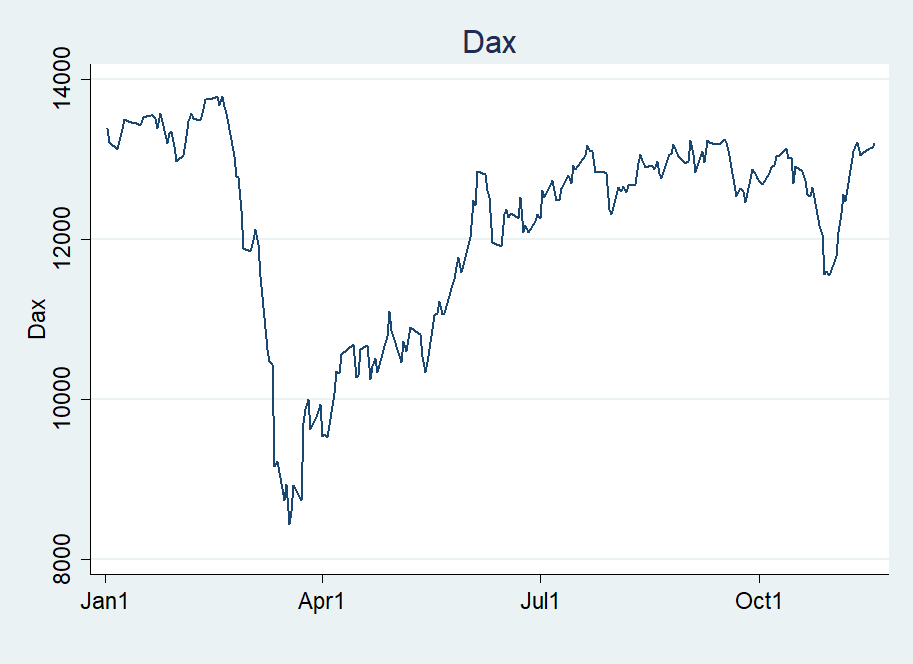
\includegraphics[height=6cm ]{\FigDir/dax.png}
	\end{figure}
	%\begin{figure}
	\centering
	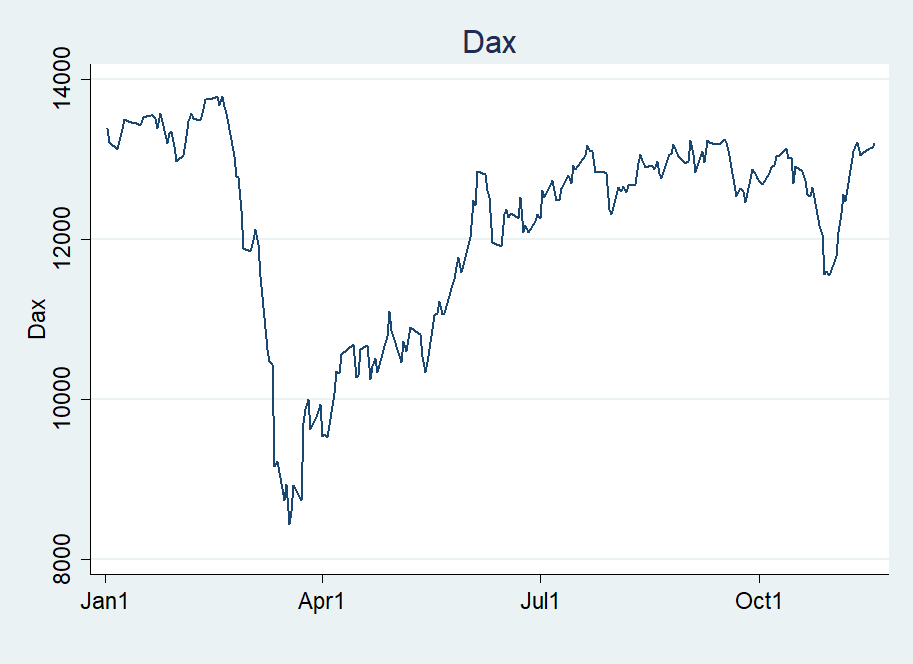
\includegraphics[height=6cm ]{\FigDir/dax.png}
\end{figure}
	%\vspace{-1em}
	\hyperlink{sp500}{\beamerbutton{S \&P 500}}
	\hyperlink{eurostoxx50}{\beamerbutton{Eurostoxx 50}}
\end{frame}

\begin{frame}[label = motivation_2]
	\frametitle{Motivation: Change of Equity Holders}
	\begin{figure}
		\centering
		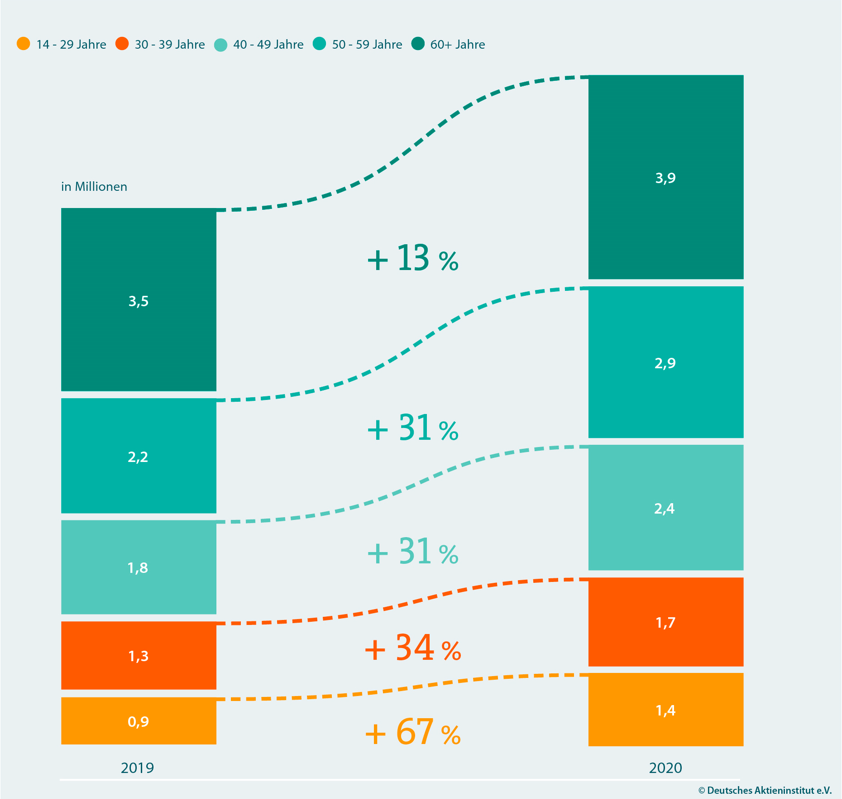
\includegraphics[height=7cm ]{\FigDir/DAI_graph.PNG}
		%\caption{Change of German Equity Holders between 2019 and 2020 by age group}
	\end{figure}
\end{frame}

\begin{frame}{This paper}
	
	\begin{block}{Research Question}
		{\begin{enumerate}
				\item What prevents households from investing?
				\item What make them invest?
				\item How are expectations and financial investments connected?
		\end{enumerate}}
	\end{block}
	\vspace{1em}
	\pause
	\begin{block}{Inserting questions in the \textit{Bundesbank Online Pilot (BOP)} I find that...}
		{
			\pause
			\begin{enumerate}
				\item \textbf{Participation costs}: lack of information and interest
				\item \textbf{Adjustment costs}: risk and time constraint
				\item \textbf{Buyers} invested either because of opportunity or savingsplan. 
				\item Higher house price and inflation \textbf{expectations} reduce the likelihood to invest
			\end{enumerate}
		}
		
	\end{block}
\end{frame}

\begin{frame}
	\frametitle{Gap in the Literature}
	\begin{enumerate}
		\item Equity Premium Puzzle: Comparing mechanisms\\
		\small{In spirit of \cite{choi_2020, bender_et_al_2019}}
		\vspace{2em}
		\item Adjustment Costs and how to overcome them\\
		\small{\cite{bonaparte_et_al_2012adjustment}}
		\vspace{2em}
		\item Expectations and Financial Asset investments\\
		\small{\cite{giglio_et_al_2019five, manski_2018survey}}
	\end{enumerate}
\end{frame}



\section{Data}

\begin{frame}
	\frametitle{Bundesbank Online Panel}
	\begin{itemize}
		\setlength\itemsep{0.8em}
		\item Bundesbank Online Pilot Survey on Consumer Expectations (BOP) 
		\item Online survey of German citizens aged 16 years or older
		\item Monthly survey with 2,000 households 
		\item Representative sample
		\item Individuals’ expectations and socio-demographic characteristics
		\pause
		\item \textbf{Additional questions on financial asset investments}
	\end{itemize} 
\end{frame}

\begin{frame}[label = Timeline]
	\frametitle{Bundesbank Online Panel}
	\vspace{-1.7em}
	\begin{figure}
		\centering
		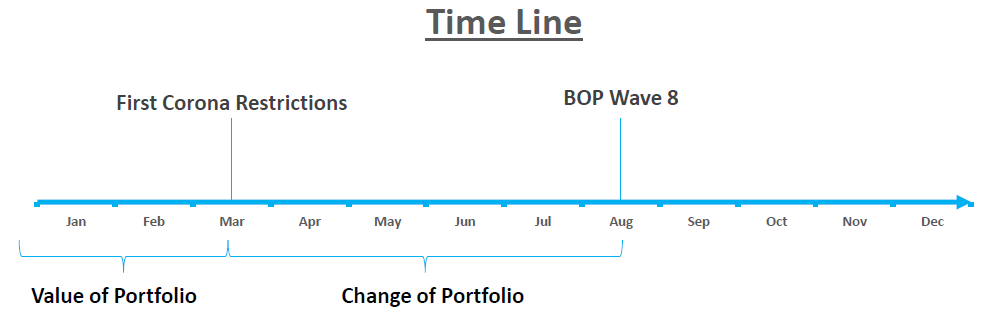
\includegraphics[scale = .45]{\FigDir/timeline_1.PNG}
	\end{figure}
	\onslide<1>{\hspace{4em}\hyperlink{BOP Q1}{\beamerbutton{BOP}}\hyperlink{BOP Q2}{\beamerbutton{BOP}}\hspace{4em}\hyperlink{BOP Q3}{\beamerbutton{BOP}}\hyperlink{BOP Q4}{\beamerbutton{BOP}}}
	\pause
	\vspace{-1.5em}
	\begin{figure}
		\centering
		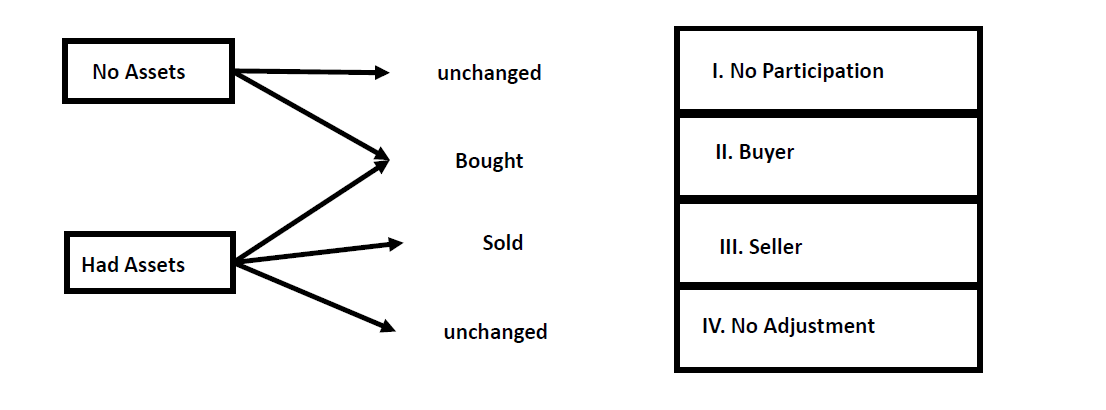
\includegraphics[scale = .45]{\FigDir/timeline_2.PNG}
	\end{figure}
\end{frame}

\begin{frame}[label = Data]
	\frametitle{Bundesbank Online Panel}
	\begin{table}[]
		\resizebox{0.9\textwidth}{!}{%
			\begin{tabular}{ccccccc}
				No   Participation &  & No Adjustment &  & Bought &  & Sold \\ 
				\hyperlink{BOP Q7}{\beamerbutton{BOP}} &  & \hyperlink{BOP Q8}{\beamerbutton{BOP}} &  & \hyperlink{BOP Q5}{\beamerbutton{BOP}} &  & \hyperlink{BOP Q6}{\beamerbutton{BOP}} \\\hline
				&  &  &  &  &  &  \\
				prices fall &  & prices fall &  & prices rise &  & prices fall \\
				&  &  &  &  &  &  \\
				too risky &  & too risky &  &  &  & too risky \\
				shock &  &  &  &  &  & shock \\
				distrust &  &  &  &  &  &  \\
				&  &  &  &  &  &  \\
				no savings &  & no savings &  & costs &  & no savings \\
				costs &  & costs &  & less consumption &  & need for consumption \\
				&  &  &  & more income &  & need debt obligations \\
				&  &  &  &  &  &  \\
				peer-effect &  & peer-effect &  & peer-effect &  & peer-effect \\
				&  &  &  &  &  &  \\
				no time &  & no time &  & time &  & no time \\
				&  &  &  &  &  &  \\
				information &  &  &  & information &  & re-balancing \\
				no   interest &  &  &  & savings plan &  &  \\
				moral &  &  &  &  &  &  \\ \hline\hline
			\end{tabular}
		}
	\end{table}
\end{frame}


\section{Results}
\begin{frame}{General Results}
	
\begin{table}[]
	\resizebox{0.9\textwidth}{!}{%
		\begin{threeparttable}
			\begin{tabular}{ll|ccccccccc}
				&  &  & \begin{tabular}[c]{@{}c@{}}no participation\\ (I)\end{tabular} &  & \begin{tabular}[c]{@{}c@{}}no adjustment\\ (II)\end{tabular} &  & \begin{tabular}[c]{@{}c@{}}bought\\ (III)\end{tabular} &  & \begin{tabular}[c]{@{}c@{}}sold\\ (IV)\end{tabular} &  \\ \hline
				Total & \% &  & \textbf{55.1} &  & \textbf{23.0} &  & \textbf{20.0} &  & \textbf{5.8} &  \\
				& \euro &  &  &  &  &  & 5,100 &  & -3,100 &  \\
				&  &  &  &  &  &  &  &  &  &  \\
				Funds & \% &  &  &  &  &  & 69.5 &  & 57.3 &  \\
				& \euro &  &  &  &  &  & 2,100 &  & -1,900 &  \\
				&  &  &  &  &  &  &  &  &  &  \\
				Bonds & \% &  &  &  &  &  & 51.5 &  & 68.4 &  \\
				& \euro &  &  &  &  &  & 2,300 &  & 0 &  \\
				&  &  &  &  &  &  &  &  &  &  \\
				Stocks & \% &  &  &  &  &  & 8.3 &  & 13.2 &  \\
				& \euro &  &  &  &  &  & 0 &  & -200 &  \\
				&  &  &  &  &  &  &  &  &  &  \\
				Other & \% &  &  &  &  &  & 17.8 &  & 29.3 &  \\
				& \euro &  &  &  &  &  & 600 &  & -1,100 &  \\ \hline
				&  &  &  &  &  &  &  &  &  &  \\
				n &  &  & 1,013 &  & 513 &  & 454 &  & 133 &   \\ \hline \hline
			\end{tabular}
		\end{threeparttable}
	}
\end{table}
\end{frame}

\begin{frame}{General Results}
	
	\begin{table}[]
		\resizebox{\textheight}{!}{%
			\begin{threeparttable}
				\begin{tabular}{l*{4}{c}}
					\hline\hline
					&\multicolumn{1}{c}{(1)}&\multicolumn{1}{c}{(2)}&\multicolumn{1}{c}{(3)}&\multicolumn{1}{c}{(4)}\\
					&\multicolumn{1}{c}{\shortstack{No \\ Participation}}&\multicolumn{1}{c}{\shortstack{No \\ Adjustment}}&\multicolumn{1}{c}{\shortstack{Has\\ Bought}}&\multicolumn{1}{c}{\shortstack{Has\\ Sold}}\\
					\hline
					&                     &                     &                     &                     \\
					college             &      -0.318\sym{***}&       0.089         &       0.292\sym{***}&       0.219\sym{*}  \\
					&     (0.086)         &     (0.096)         &     (0.094)         &     (0.124)         \\
					[1em]
					female              &       0.287\sym{***}&       0.069         &      -0.467\sym{***}&      -0.370\sym{***}\\
					&     (0.082)         &     (0.096)         &     (0.087)         &     (0.123)         \\
					[1em]
					$<30$               &      -0.052         &      -0.216         &       0.360\sym{***}&       0.183         \\
					&     (0.129)         &     (0.176)         &     (0.128)         &     (0.176)         \\
					[1em]
					owner               &      -0.381\sym{***}&       0.307\sym{***}&       0.240\sym{***}&      -0.116         \\
					&     (0.086)         &     (0.101)         &     (0.092)         &     (0.134)         \\
					[1em]
					fin illiterate &       0.457\sym{***}&      -0.218         &      -0.596\sym{***}&      -0.047         \\
					&     (0.153)         &     (0.190)         &     (0.157)         &     (0.190)         \\
					\hline
					Observations        &        2022         &        2022         &        2022         &        2022         \\
					Controls            &         Yes         &         Yes         &         Yes         &         Yes         \\
					\hline\hline
				\end{tabular}
			\end{threeparttable}
		}
	\end{table}

\end{frame}

\begin{frame}{General Results}
	
	\begin{table}[]
		\resizebox{0.7\textwidth}{!}{%
			\begin{threeparttable}
				\begin{tabular}{l*{4}{c}}
					\hline\hline
					&\multicolumn{1}{c}{(1)}&\multicolumn{1}{c}{(2)}&\multicolumn{1}{c}{(3)}&\multicolumn{1}{c}{(4)}\\
					&\multicolumn{1}{c}{\shortstack{No \\ Participation}}&\multicolumn{1}{c}{\shortstack{No \\ Adjustment}}&\multicolumn{1}{c}{\shortstack{Has\\ Bought}}&\multicolumn{1}{c}{\shortstack{Has\\ Sold}}\\
					\hline
					&                     &                     &                     &                     \\
					full-time           &      -0.236         &      -0.034         &       0.402\sym{**} &       0.375\sym{*}  \\
					&     (0.145)         &     (0.173)         &     (0.162)         &     (0.218)         \\
					[1em]
					part-time           &      -0.120         &       0.014         &       0.254         &       0.401         \\
					&     (0.185)         &     (0.237)         &     (0.204)         &     (0.273)         \\
					[1em]
					retired             &      -0.102         &       0.019         &       0.132         &       0.405\sym{*}  \\
					&     (0.159)         &     (0.185)         &     (0.177)         &     (0.244)         \\
					[1em]
					self-employed       &      -0.075         &      -0.086         &       0.190         &       0.626\sym{**} \\
					&     (0.226)         &     (0.245)         &     (0.228)         &     (0.289)         \\
					[1em]
					$<1500$\euro            &       0.420\sym{***}&      -0.279\sym{*}  &      -0.568\sym{***}&       0.033         \\
					&     (0.141)         &     (0.148)         &     (0.183)         &     (0.209)         \\
					\hline
					Observations        &        2022         &        2022         &        2022         &        2022         \\
					Controls            &         Yes         &         Yes         &         Yes         &         Yes         \\
					\hline\hline
				\end{tabular}
			\end{threeparttable}
		}
	\end{table}
	
\end{frame}

\begin{frame}[label = results_nopart]
	\frametitle{No Participation}
	\pause
	\begin{table}[]
		%\caption{Summary Statistics: Reasons No Participation}
		\label{tab:reason_nostocks}
		\resizebox{0.9\textwidth}{!} &  & 72.80\% &  & 3.25 &  & 0.58 \\
					\textbf{no interest} &  & \textbf{47.49\%} &  & 69.88\% &  & 3.17 &  & 0.47 \\
					distrust &  & 37.99\% &  & 63.03\% &  & 3.00 &  & 0.27 \\
					too risky &  & 34.77\% &  & 59.35\% &  & 2.88 &  & 0.17 \\
					no time &  & 33.37\% &  & 57.89\% &  & 2.83 &  & 0.09 \\
					peer-effect &  & 30.22\% &  & 51.31\% &  & 2.70 &  & -0.08 \\
					no savings &  & 30.32\% &  & 53.92\% &  & 2.73 &  & -0.12 \\
					prices fall &  & 17.52\% &  & 51.77\% &  & 2.61 &  & -0.15 \\
					shock &  & 23.91\% &  & 46.28\% &  & 2.53 &  & -0.22 \\
					costs &  & 19.95\% &  & 42.88\% &  & 2.44 &  & -0.34 \\
					moral &  & 16.27\% &  & 32.39\% &  & 2.17 &  & -0.70\\ 
					&  &  &  &  &  &  &  &  \\\hline \hline
				\end{tabular}
			\end{threeparttable}
		}
	\end{table}
	\hyperlink{regression_nopart_dem}{\beamerbutton{Demo}}
\end{frame}

\begin{frame}
	\frametitle{No Participation: PCA}
	\begin{table}[]
		\resizebox{0.9\textwidth}{!}{%
			\begin{threeparttable}
				\begin{tabular}{lcclcclc}
					\hline
					\multicolumn{2}{c}{\begin{tabular}[c]{@{}c@{}}Comp   1\\ \onslide<2->{risk aversion}\end{tabular}} &  & \multicolumn{2}{c}{\begin{tabular}[c]{@{}c@{}}Comp   2\\ \onslide<3->{lack of resources}\end{tabular}} &  & \multicolumn{2}{c}{\begin{tabular}[c]{@{}c@{}}Comp   3\\ \onslide<4->{lack of savings}\end{tabular}} \\ \cline{1-2} \cline{4-5} \cline{7-8} 
					&  &  &  &  &  &  &  \\
					\onslide<2->{too risky & 0.42} &  & \onslide<3->{no interest & 0.47} &  & \onslide<4->{no savings & 0.64} \\
					\onslide<2->{distrust & 0.42} &  & \onslide<3->{information & 0.40} &  & \onslide<4->{moral & -0.60} \\
					\onslide<2->{shock & 0.37} &  & \onslide<3->{no time & 0.40} &  &  &  \\
					\onslide<2->{prices fall & 0.35} &  & \onslide<3->{no savings & 0.34} &  &  &  \\
					&  &  & \onslide<3->{shock & -0.33} &  &  &  \\
					&  &  &  &  &  &  &  \\ \hline \hline
				\end{tabular}
			\end{threeparttable}
		}
	\end{table}
\end{frame}


\begin{frame}[label = regression_pca_noadjust_dem]
	\frametitle{No Participation: PCA}
	\begin{table}[] \centering
		\resizebox{0.7\textwidth}{!}{%
			\begin{threeparttable}
				\begin{tabular}{l*{6}c}
					\hline\hline
					                    &            &\multicolumn{1}{c}{(1)}&            &\multicolumn{1}{c}{(2)}&            &\multicolumn{1}{c}{(3)}\\
                    &            &\multicolumn{1}{c}{\shortstack{Risk \\ Aversion}}&            &\multicolumn{1}{c}{\shortstack{Lack of \\ Resources}}&            &\multicolumn{1}{c}{\shortstack{Lack of\\ Savings}}\\
\hline
age                 &            &       0.006\sym{***}&            &      -0.009\sym{***}&            &      -0.002         \\
                    &            &     (0.002)         &            &     (0.002)         &            &     (0.003)         \\
[1em]
$<1500$             &            &      -0.073         &            &       0.029         &            &       0.261\sym{***}\\
                    &            &     (0.058)         &            &     (0.064)         &            &     (0.096)         \\
\hline
Observations        &            &         811         &            &         823         &            &         827         \\
Adjusted \(R^{2}\)  &            &       0.073         &            &       0.103         &            &       0.059         \\
Controls            &            &         Yes         &            &         Yes         &            &         Yes         \\

					\hline\hline
				\end{tabular}
			\end{threeparttable}
		}
	\end{table}
	\hyperlink{regression_pca_noadjust_dem_control}{\beamerbutton{Controls}}
\end{frame}


\begin{frame}
	\frametitle{No Participation}
	\begin{block}{Takeaway \#1: No Participation}
		{
			\begin{enumerate}
				\item Lack of information and interest are dominant factors
				\item Importance of risk increases with age, lack of resources decrease in age, and lack of savings decreases with income
			\end{enumerate}
		}
	\end{block}
	
\end{frame}

\begin{frame}[label=results_noadjust]
	\frametitle{No Adjustment}
	\pause
	\begin{table}[]
		\resizebox{\textwidth}{!}{%
			\begin{threeparttable}
				\begin{tabular}{l|lccccccc}
					&  & \begin{tabular}[c]{@{}c@{}}Fully agree\\ (I)\end{tabular} &  & \begin{tabular}[c]{@{}c@{}}At least\\ rather agree\\ (II)\end{tabular} &  & \begin{tabular}[c]{@{}c@{}}Mean\\ (III)\end{tabular} &  & \begin{tabular}[c]{@{}c@{}}Standardized\\ (III)\end{tabular} \\ \hline
					&  &  &  &  &  &  &  &  \\
					too risky &  & 20.47\% &  & 55.52\% &  & 2.53 &  & 0.31 \\
					no time &  & 17.05\% &  & 49.39\% &  & 2.38 &  & 0.11 \\
					prices fall &  & 9.47\% &  & 48.62\% &  & 2.39 &  & 0.09 \\
					no savings &  & 18.25\% &  & 42.20\% &  & 2.30 &  & -0.06 \\
					peer-effect &  & 17.24\% &  & 36.07\% &  & 2.12 &  & -0.19 \\
					costs &  & 10.67\% &  & 32.40\% &  & 2.09 &  & -0.28 \\ 
					&  &  &  &  &  &  &  &  \\\hline \hline
				\end{tabular}
			\end{threeparttable}
		}
	\end{table}
	\hyperlink{regression_noadjust_dem}{\beamerbutton{Demo}}
\end{frame}

\begin{frame}
	\frametitle{No Adjustment: PCA}
	\begin{table}[]
		% \caption{ Principal Component Analysis: No Adjustment}
		% \label{tab:reason_unchanged}
		\resizebox{0.7\textwidth}{!}{%
			\begin{threeparttable}
				\begin{tabular}{llcll}
					\hline
					\multicolumn{2}{c}{\begin{tabular}[c]{@{}c@{}}Comp   1\\ bad timing\end{tabular}} &  & \multicolumn{2}{c}{\begin{tabular}[c]{@{}c@{}}Comp   2\\ time constraint\end{tabular}} \\ \cline{1-2} \cline{4-5} 
					& \multicolumn{1}{c}{} &  &  & \multicolumn{1}{c}{} \\
					too risky & 0.63 &  & no savings & -0.70 \\
					prices fall & 0.58 &  & peer effect & 0.55 \\
					costs & 0.49 &  & no time & 0.45 \\
					&  &  &  &  \\ \hline \hline
				\end{tabular}
			\end{threeparttable}
		}
	\end{table}
\end{frame}

\begin{frame}
	\frametitle{No Adjustment}
	\begin{block}{Takeaway \#2: No Adjustment}
		{
			\begin{enumerate}
				\item Risk, time, and prices fall are dominant factors
				\item Either bad timing or time constraint
				\item Needs more research
			\end{enumerate}
		}
	\end{block}
	
\end{frame}

\begin{frame}[label = results_bought]
	\frametitle{Buyer}
	\pause
	\begin{table}[]
		\resizebox{\textwidth}{!} &  & 62.07\% &  & 2.76 &  & 0.92 \\
					\textbf{prices rise} &  & \textbf{38.74\%} &  & 64.08\% &  & 2.79 &  & 0.90 \\
					time &  & 8.09\% &  & 26.59\% &  & 1.77 &  & -0.07 \\
					information &  & 7.60\% &  & 24.22\% &  & 1.70 &  & -0.15 \\
					less   consumption &  & 3.88\% &  & 18.73\% &  & 1.58 &  & -0.29 \\
					more income &  & 4.33\% &  & 19.88\% &  & 1.57 &  & -0.31 \\
					peer-effect &  & 4.15\% &  & 13.87\% &  & 1.49 &  & -0.36 \\
					bank fees &  & 0.38\% &  & 3.52\% &  & 1.21 &  & -0.65 \\ 
					&  &  &  &  &  &  &  &  \\\hline \hline
				\end{tabular}
			\end{threeparttable}
		}
	\end{table}
	\hyperlink{regression_bought_dem}{\beamerbutton{Demo}}
\end{frame}

\begin{frame}
	\frametitle{Buyer: active vs passive}
	
	\begin{table}[]
		\resizebox{1.2\textheight}{!}{%
			\begin{tabular}{l*{3}{c}}
				\hline
				%                    &\multicolumn{1}{c}{(1)}&\multicolumn{1}{c}{(2)}\\
                    &\multicolumn{1}{c}{\shortstack{active}}&\multicolumn{1}{c}{\shortstack{passive}}\\
\hline
                    &                     &                     \\
owner               &       0.518\sym{***}&      -0.375\sym{*}  \\
                    &     (0.196)         &     (0.192)         \\
[1em]
$<30$               &       0.639\sym{**} &      -0.337         \\
                    &     (0.257)         &     (0.261)         \\
[1em]
first time          &       0.637\sym{*}  &      -0.743\sym{**} \\
                    &     (0.353)         &     (0.353)         \\
[1em]
bought \& sold      &       0.711\sym{***}&      -0.847\sym{***}\\
                    &     (0.208)         &     (0.206)         \\
\hline
Observations        &         454         &         454         \\
Controls            &         Yes         &         Yes         \\

				                    &\multicolumn{1}{c}{(1)}&\multicolumn{1}{c}{(2)}\\
				&\multicolumn{1}{c}{\shortstack{active}}&\multicolumn{1}{c}{\shortstack{passive}}\\
				\hline
				&                     &                     \\
				owner               &       \textbf{0.565\sym{***}}&      -0.401\sym{**} \\
				&     (0.196)         &     (0.192)         \\
				[1em]
				$<30$               &       \textbf{0.624\sym{**}} &      -0.347         \\
				&     (0.254)         &     (0.261)         \\
				[1em]
				first time          &       \textbf{0.627\sym{*}}  &      -0.744\sym{**} \\
				&     (0.351)         &     (0.353)         \\
				[1em]
				bought \& sold      &       \textbf{0.669\sym{***}}&      -0.818\sym{***}\\
				&     (0.206)         &     (0.206)         \\
				&&\\
				&&\\
				&&\\
				&&\\
				&&\\
				&&\\
				\hline
				Observations        &         454         &         454         \\
				Controls            &         Yes         &         Yes         \\
				\hline\hline
			\end{tabular}
			\hspace{4em}
			\pause
			\begin{tabular}{l*{3}{c}}
				\hline
				%                    &\multicolumn{1}{c}{(1)}&\multicolumn{1}{c}{(2)}\\
                    &\multicolumn{1}{c}{\shortstack{active}}&\multicolumn{1}{c}{\shortstack{passive}}\\
\hline
main                &                     &                     \\
time                &       0.703\sym{***}&      -1.152\sym{***}\\
                    &     (0.126)         &     (0.136)         \\
[1em]
information         &       0.206\sym{*}  &      -0.899\sym{***}\\
                    &     (0.121)         &     (0.128)         \\
[1em]
less consumption    &       0.224         &      -0.820\sym{***}\\
                    &     (0.170)         &     (0.167)         \\
[1em]
more income         &       0.415\sym{**} &      -1.120\sym{***}\\
                    &     (0.172)         &     (0.157)         \\
[1em]
costs               &       0.871\sym{***}&      -2.069\sym{***}\\
                    &     (0.270)         &     (0.301)         \\
[1em]
peer effect         &       0.742\sym{***}&      -1.534\sym{***}\\
                    &     (0.166)         &     (0.170)         \\
\hline
Observations        &         431         &         431         \\
Controls            &         Yes         &         Yes         \\

				                    &\multicolumn{1}{c}{(1)}&\multicolumn{1}{c}{(2)}\\
				&\multicolumn{1}{c}{\shortstack{active}}&\multicolumn{1}{c}{\shortstack{passive}}\\
				\hline
				&                     &                     \\
				time                &       \textbf{0.703\sym{***}}&      -1.152\sym{***}\\
				&     (0.126)         &     (0.136)         \\
				[1em]
				information         &       \textbf{0.206\sym{*}}  &      -0.899\sym{***}\\
				&     (0.121)         &     (0.128)         \\
				[1em]
				less consumption    &       0.224         &      -0.820\sym{***}\\
				&     (0.170)         &     (0.167)         \\
				[1em]
				more income         &       \textbf{0.415\sym{**}} &      -1.120\sym{***}\\
				&     (0.172)         &     (0.157)         \\
				[1em]
				costs               &       \textbf{0.871\sym{***}}&      -2.069\sym{***}\\
				&     (0.270)         &     (0.301)         \\
				[1em]
				peer effect         &       \textbf{0.742\sym{***}}&      -1.534\sym{***}\\
				&     (0.166)         &     (0.170)         \\
				\hline
				Observations        &         431         &         431         \\
				Controls            &         Yes         &         Yes         \\
				\hline\hline
			\end{tabular}
			
		}
	\end{table}
	
\end{frame}

\begin{frame}{Buyer: By asset type}
	\begin{table}[]
		\centering
		\resizebox{0.7\textwidth}{!}{
			\begin{threeparttable}
				\begin{tabular}{l|ccccccccc}
					%                    &            &\multicolumn{1}{c}{(1)}&            &\multicolumn{1}{c}{(2)}&            &\multicolumn{1}{c}{(3)}&            &\multicolumn{1}{c}{(4)}\\
                    &            &\multicolumn{1}{c}{\shortstack{funds}}&            &\multicolumn{1}{c}{\shortstack{Bonds}}&            &\multicolumn{1}{c}{\shortstack{Stocks}}&            &\multicolumn{1}{c}{\shortstack{Other}}\\
\hline
                    &            &                     &            &                     &            &                     &            &                     \\
has funds           &            &       2.527\sym{***}&            &      -0.699\sym{**} &            &       1.219\sym{**} &            &      -0.771\sym{*}  \\
                    &            &     (0.317)         &            &     (0.327)         &            &     (0.553)         &            &     (0.408)         \\
[1em]
has Bonds           &            &       0.063         &            &       1.432\sym{***}&            &       0.538         &            &       0.036         \\
                    &            &     (0.341)         &            &     (0.263)         &            &     (0.399)         &            &     (0.382)         \\
[1em]
has Stocks          &            &      -0.241         &            &       0.203         &            &       2.192\sym{***}&            &      -0.057         \\
                    &            &     (0.380)         &            &     (0.389)         &            &     (0.395)         &            &     (0.490)         \\
[1em]
has Other           &            &      -0.321         &            &       0.901\sym{***}&            &       0.150         &            &       2.027\sym{***}\\
                    &            &     (0.329)         &            &     (0.325)         &            &     (0.427)         &            &     (0.349)         \\
[1em]
first time          &            &       0.570         &            &       1.098\sym{***}&            &       0.000         &            &       0.900\sym{*}  \\
                    &            &     (0.414)         &            &     (0.379)         &            &         (.)         &            &     (0.461)         \\
[1em]
bought \& sold      &            &      -0.419\sym{*}  &            &       0.452         &            &      -0.598\sym{*}  &            &      -0.139         \\
                    &            &     (0.222)         &            &     (0.276)         &            &     (0.326)         &            &     (0.316)         \\
\hline
Observations        &            &         454         &            &         454         &            &         430         &            &         454         \\
Controls            &            &         Yes         &            &         Yes         &            &         Yes         &            &         Yes         \\

					                    &            &\multicolumn{1}{c}{(1)}&            &\multicolumn{1}{c}{(2)}&            &\multicolumn{1}{c}{(3)}&            &\multicolumn{1}{c}{(4)}\\
					&            &\multicolumn{1}{c}{\shortstack{Funds}}&            &\multicolumn{1}{c}{\shortstack{Bonds}}&            &\multicolumn{1}{c}{\shortstack{Stocks}}&            &\multicolumn{1}{c}{\shortstack{Other}}\\
					\hline
					&            &                     &            &                     &            &                     &            &                     \\
					has Funds           &            &       \onslide<2->{\textbf{2.527\sym{***}}&            &      -0.699\sym{**} &            &       1.219\sym{**} &            &      -0.771\sym{*}}  \\
					&            &     \onslide<2->{(0.317)         &            &     (0.327)         &            &     (0.553)         &            &     (0.408)}         \\
					[1em]
					has Bonds           &            &       \onslide<2->{0.063         &            &       \textbf{1.432\sym{***}}&            &       0.538         &            &       0.036}         \\
					&            &     \onslide<2->{(0.341)         &            &     (0.263)         &            &     (0.399)         &            &     (0.382)}         \\
					[1em]
					has Stocks          &            &      \onslide<2->{-0.241         &            &       0.203         &            &       \textbf{2.192\sym{***}}&            &      -0.057}         \\
					&            &     \onslide<2->{(0.380)         &            &     (0.389)         &            &     (0.395)         &            &     (0.490)}         \\
					[1em]
					has Other           &            &      \onslide<2->{-0.321         &            &       0.901\sym{***}&            &       0.150         &            &       \textbf{2.027\sym{***}}}\\
					&            &     \onslide<2->{(0.329)         &            &     (0.325)         &            &     (0.427)         &            &     (0.349)}         \\
					[1em]
					first time          &            &       \onslide<2->{0.570         &            &       1.098\sym{***}&            &       0.000         &            &       0.900\sym{*}}  \\
					&            &     \onslide<2->{(0.414)         &            &     (0.379)         &            &         (.)         &            &     (0.461)}         \\
					[1em]
					bought \& sold      &            &      \onslide<2->{-0.419\sym{*}  &            &       0.452         &            &      -0.598\sym{*}  &            &      -0.139}         \\
					&            &     \onslide<2->{(0.222)         &            &     (0.276)         &            &     (0.326)         &            &     (0.316)}         \\
					\hline
					Observations        &            &         454         &            &         454         &            &         430         &            &         454         \\
					Controls            &            &         Yes         &            &         Yes         &            &         Yes         &            &         Yes         \\
					
					\hline \hline
				\end{tabular}
			\end{threeparttable}
		}
	\end{table}
\end{frame}

\begin{frame}{Buyer: By asset type}
	\begin{table}[]
		\centering
		\resizebox{0.7\textwidth}{!}{
			\begin{threeparttable}
				\begin{tabular}{l|ccccccccc}
					%                    &            &\multicolumn{1}{c}{(1)}&            &\multicolumn{1}{c}{(2)}&            &\multicolumn{1}{c}{(3)}&            &\multicolumn{1}{c}{(4)}\\
                    &            &\multicolumn{1}{c}{\shortstack{funds}}&            &\multicolumn{1}{c}{\shortstack{Bonds}}&            &\multicolumn{1}{c}{\shortstack{Stocks}}&            &\multicolumn{1}{c}{\shortstack{Other}}\\
\hline
                    &            &                     &            &                     &            &                     &            &                     \\
value funds         &            &       0.108\sym{**} &            &      -0.085\sym{*}  &            &      -0.127\sym{*}  &            &      -0.021         \\
                    &            &     (0.047)         &            &     (0.051)         &            &     (0.070)         &            &     (0.059)         \\
[1em]
value bonds         &            &      -0.143\sym{**} &            &       0.206\sym{***}&            &      -0.040         &            &      -0.191\sym{***}\\
                    &            &     (0.061)         &            &     (0.051)         &            &     (0.075)         &            &     (0.067)         \\
[1em]
value stocks        &            &       0.010         &            &      -0.032         &            &       0.045         &            &      -0.035         \\
                    &            &     (0.079)         &            &     (0.079)         &            &     (0.067)         &            &     (0.104)         \\
[1em]
value other         &            &      -0.088         &            &      -0.142\sym{**} &            &      -0.170         &            &       0.193\sym{***}\\
                    &            &     (0.062)         &            &     (0.062)         &            &     (0.112)         &            &     (0.071)         \\
\hline
Observations        &            &         454         &            &         454         &            &         430         &            &         454         \\
Controls            &            &         Yes         &            &         Yes         &            &         Yes         &            &         Yes         \\

					                    &            &\multicolumn{1}{c}{\shortstack{Funds}}&            &\multicolumn{1}{c}{\shortstack{Bonds}}&            &\multicolumn{1}{c}{\shortstack{Stocks}}&            &\multicolumn{1}{c}{\shortstack{Other}}\\
					\hline
					&            &                     &            &                     &            &                     &            &                     \\
					value funds         &            &       \textbf{0.108\sym{**}} &            &      -0.085\sym{*}  &            &      -0.127\sym{*}  &            &      -0.021         \\
					&            &     (0.047)         &            &     (0.051)         &            &     (0.070)         &            &     (0.059)         \\
					[1em]
					value bonds         &            &      -0.143\sym{**} &            &       \textbf{0.206\sym{***}}&            &      -0.040         &            &      -0.191\sym{***}\\
					&            &     (0.061)         &            &     (0.051)         &            &     (0.075)         &            &     (0.067)         \\
					[1em]
					value stocks        &            &       0.010         &            &      -0.032         &            &       0.045         &            &      -0.035         \\
					&            &     (0.079)         &            &     (0.079)         &            &     (0.067)         &            &     (0.104)         \\
					[1em]
					value other         &            &      -0.088         &            &      -0.142\sym{**} &            &      -0.170         &            &       \textbf{0.193\sym{***}}\\
					&            &     (0.062)         &            &     (0.062)         &            &     (0.112)         &            &     (0.071)         \\
					\hline
					Observations        &            &         454         &            &         454         &            &         430         &            &         454         \\
					Controls            &            &         Yes         &            &         Yes         &            &         Yes         &            &         Yes         \\
					\hline \hline
				\end{tabular}
			\end{threeparttable}
		}
	\end{table}
\end{frame}

\begin{frame}
	\frametitle{Buyer}
	\begin{block}{Takeaway \#3: Buyer}
		{
			\begin{enumerate}
				\item Active vs Passive buyers
				\item Active buyers are younger, richer and respond to additional information, time, income, costs, and peer effects.
				\item Respondents bought the asset type they already held
			\end{enumerate}
		}
	\end{block}
\end{frame}

\begin{frame}
	\frametitle{Expectations and Buyer}
	Here is a equation:
	I run probit regressions of the form:
%	\begin{verbatimwrite}{\EqDir/Prob_regression_expec}
%		\begin{align}
%			y_i = \beta X + \gamma Z + \epsilon  \label{eq:Prob_reg_expec}
%		\end{align}
%	\end{verbatimwrite}
		\begin{align}
		y_i = \beta X + \gamma Z + \epsilon  \label{eq:Prob_reg_expec}
	\end{align}

\end{frame}


\begin{frame}[label = regression_bought_expec_pp]
	\frametitle{House Price Expectations and Buyer}
	\vspace{-1em}
	\begin{table}[htbp]\centering
		\resizebox{\textwidth}{!}{%
			\begin{tabular}{l*{6}{c}}
				\hline\hline
				%                    &\multicolumn{1}{c}{(1)}&\multicolumn{1}{c}{(2)}&\multicolumn{1}{c}{(3)}&\multicolumn{1}{c}{(4)}&\multicolumn{1}{c}{(5)}&\multicolumn{1}{c}{(6)}\\
                    &\multicolumn{1}{c}{\shortstack{All}}&\multicolumn{1}{c}{\shortstack{Owner}}&\multicolumn{1}{c}{\shortstack{Renter}}&\multicolumn{1}{c}{\shortstack{All}}&\multicolumn{1}{c}{\shortstack{Owner}}&\multicolumn{1}{c}{\shortstack{Renter}}\\
\hline
                    &                     &                     &                     &                     &                     &                     \\
housing quali       &      -0.198\sym{***}&                     &                     &                     &                     &                     \\
                    &     (0.051)         &                     &                     &                     &                     &                     \\
[1em]
prop quali          &                     &      -0.152\sym{***}&                     &                     &                     &                     \\
                    &                     &     (0.055)         &                     &                     &                     &                     \\
[1em]
rent quali          &                     &                     &      -0.143\sym{*}  &                     &                     &                     \\
                    &                     &                     &     (0.080)         &                     &                     &                     \\
[1em]
house price wins    &                     &                     &                     &      -0.026\sym{***}&      -0.011         &      -0.048\sym{***}\\
                    &                     &                     &                     &     (0.008)         &     (0.010)         &     (0.014)         \\
\hline
Observations        &        2012         &        1257         &         755         &        1871         &        1171         &         700         \\
Controls            &         Yes         &         Yes         &         Yes         &         Yes         &         Yes         &         Yes         \\

				&\multicolumn{1}{c}{(1)}&\multicolumn{1}{c}{(2)}&\multicolumn{1}{c}{(3)}&\multicolumn{1}{c}{(4)}&\multicolumn{1}{c}{(5)}&\multicolumn{1}{c}{(6)}\\
				&\multicolumn{1}{c}{\shortstack{All}}&\multicolumn{1}{c}{\shortstack{Owner}}&\multicolumn{1}{c}{\shortstack{Renter}}&\multicolumn{1}{c}{\shortstack{All}}&\multicolumn{1}{c}{\shortstack{Owner}}&\multicolumn{1}{c}{\shortstack{Renter}}\\
				\hline
				&                     &                     &                     &                     &                     &                     \\
				housing quali       &      \onslide<2->{-0.195\sym{***}}&                     &                     &                     &                     &                     \\
				&     \onslide<2->{(0.050)}         &                     &                     &                     &                     &                     \\
				[1em]
				prop quali          &                     &      \onslide<3->{-0.146\sym{***}}&                     &                     &                     &                     \\
				&                     &     \onslide<3->{(0.055)}         &                     &                     &                     &                     \\
				[1em]
				rent quali          &                     &                     &      \onslide<3->{-0.150\sym{*}}  &                     &                     &                     \\
				&                     &                     &     \onslide<3->{(0.079)}         &                     &                     &                     \\
				[1em]
				house price PE    &                     &                     &                     &      \onslide<4->{-0.026\sym{***}}&      \onslide<4->{-0.011}         &      \onslide<4->{-0.049\sym{***}}\\
				&                     &                     &                     &     \onslide<4->{(0.008)}         &     \onslide<4->{(0.010)}         &     \onslide<4->{(0.014)}         \\
				\hline
				Observations        &        2019         &        1263         &         759         &        1880         &        1176         &         704         \\
				Controls            &         Yes         &         Yes         &         Yes         &         Yes         &         Yes         &         Yes         \\
				\hline\hline
			\end{tabular}
		}
	\end{table}
	\hyperlink{regression_bought_expec_pp_cond}{\beamerbutton{Conditional on Stockholdings}}
\end{frame}

\begin{frame}[label = regression_bought_expec_infl]
	\frametitle{Inflation Expectations and Buyer}
	\vspace{-1em}
	\begin{table}[htbp]\centering
		\resizebox{0.9\textwidth}{!}{%
			\begin{tabular}{l*{8}{c}}
				\hline\hline
				%                    &\multicolumn{1}{c}{(1)}         &\multicolumn{1}{c}{(2)}         &\multicolumn{1}{c}{(3)}         &\multicolumn{1}{c}{(4)}         &\multicolumn{1}{c}{(5)}         &\multicolumn{1}{c}{(6)}         &\multicolumn{1}{c}{(7)}         &\multicolumn{1}{c}{(8)}         \\
\hline
                    &                     &                     &                     &                     &                     &                     &                     &                     \\
inflation quali     &      -0.231\sym{***}&                     &                     &                     &                     &                     &                     &                     \\
                    &     (0.074)         &                     &                     &                     &                     &                     &                     &                     \\
[1em]
inflation PE wins   &                     &      -0.100\sym{***}&      -0.099\sym{***}&      -0.095\sym{***}&                     &                     &                     &                     \\
                    &                     &     (0.019)         &     (0.019)         &     (0.020)         &                     &                     &                     &                     \\
[1em]
fin illiterate:     &                     &                     &      -0.363         &                     &                     &                     &                     &                     \\
inflation $>|30|$   &                     &                     &     (0.230)         &                     &                     &                     &                     &                     \\
[1em]
fin illiterate:     &                     &                     &                     &      -0.176         &                     &                     &                     &                     \\
inflation $>|10|$   &                     &                     &                     &     (0.217)         &                     &                     &                     &                     \\
[1em]
$0<$ inflation $<10$&                     &                     &                     &                     &      -0.118\sym{***}&                     &                     &                     \\
                    &                     &                     &                     &                     &     (0.025)         &                     &                     &                     \\
[1em]
$0<$ inflation $<5$ &                     &                     &                     &                     &                     &      -0.146\sym{***}&                     &                     \\
                    &                     &                     &                     &                     &                     &     (0.034)         &                     &                     \\
[1em]
inflation prob exp  &                     &                     &                     &                     &                     &                     &      -0.049\sym{***}&      -0.090\sym{***}\\
                    &                     &                     &                     &                     &                     &                     &     (0.017)         &     (0.020)         \\
[1em]
inflation prob sd   &                     &                     &                     &                     &                     &                     &                     &      -0.582\sym{***}\\
                    &                     &                     &                     &                     &                     &                     &                     &     (0.193)         \\
\hline
Observations        &        2011         &        1873         &        1873         &        1873         &        1817         &        1655         &        1710         &        1710         \\
Controls            &         Yes         &         Yes         &         Yes         &         Yes         &         Yes         &         Yes         &         Yes         &         Yes         \\

				                    &\multicolumn{1}{c}{(1)}         &\multicolumn{1}{c}{(2)}         &\multicolumn{1}{c}{(3)}         &\multicolumn{1}{c}{(4)}         &\multicolumn{1}{c}{(5)}         &\multicolumn{1}{c}{(6)}         &\multicolumn{1}{c}{(7)}         &\multicolumn{1}{c}{(8)}         \\
				\hline
				&                     &                     &                     &                     &                     &                     &                     &                     \\
				inflation quali     &       \onslide<2->{-0.235\sym{***}}&                     &                     &                     &                     &                     &                     &                     \\
				&      \onslide<2->{(0.073)}         &                     &                     &                     &                     &                     &                     &                     \\
				[1em]
				inflation PE   &                     &      \onslide<3->{-0.098\sym{***}}&      \onslide<4->{-0.097\sym{***}}&      \onslide<4->{-0.093\sym{***}}&                     &                     &                     &                     \\
				&                     &     \onslide<3->{(0.019)}         &     \onslide<4->{(0.018)}         &     \onslide<4->{(0.020)}         &                     &                     &                     &                     \\
				[1em]
				fin illiterate:     &                     &                     &      \onslide<4->{-0.366}         &                     &                     &                     &                     &                     \\
				inflation $>|30|$   &                     &                     &     \onslide<4->{(0.227)}         &                     &                     &                     &                     &                     \\
				[1em]
				fin illiterate:     &                     &                     &                     &      \onslide<4->{-0.183}         &                     &                     &                     &                     \\
				inflation $>|10|$   &                     &                     &                     &     \onslide<4->{(0.214)}         &                     &                     &                     &                     \\
				[1em]
				$0<$ inflation $<10$&                     &                     &                     &                     &      \onslide<5->{-0.116\sym{***}}&                     &                     &                     \\
				&                     &                     &                     &                     &     \onslide<5->{(0.025)}         &                     &                     &                     \\
				[1em]
				$0<$ inflation $<5$ &                     &                     &                     &                     &                     &      \onslide<5->{-0.141\sym{***}}&                     &                     \\
				&                     &                     &                     &                     &                     &     \onslide<5->{(0.034)}         &                     &                     \\
				[1em]
				inflation prob exp  &                     &                     &                     &                     &                     &                     &      \onslide<6->{-0.049\sym{***}}&      \onslide<6->{-0.088\sym{***}}\\
				&                     &                     &                     &                     &                     &                     &     \onslide<6->{(0.017)}         &     \onslide<6->{(0.019)}         \\
				[1em]
				inflation prob std   &                     &                     &                     &                     &                     &                     &                     &      \onslide<6->{-0.564\sym{***}}\\
				&                     &                     &                     &                     &                     &                     &                     &     \onslide<6->{(0.191)}         \\
				\hline
				Observations        &        2018         &        1883         &        1883         &        1883         &        1827         &        1663         &        1720         &        1720         \\
				Controls            &         Yes         &         Yes         &         Yes         &         Yes         &         Yes         &         Yes         &         Yes         &         Yes         \\
				\hline\hline
			\end{tabular}
		}
	\end{table}
	\hyperlink{regression_bought_infl_cond}{\beamerbutton{Conditional on Stockholdings}}\hyperlink{regression_expec_infl}{\beamerbutton{interest rate vs inverted PC}}
\end{frame}

\begin{frame}{Expectations and Buyer}
	\begin{block}{Takeaway \#4: Expectations}
		{
			\begin{enumerate}
				\item Higher houseprice expectations crowds out financial asset investments
				\item Higher inflation expectations reduces probability to buy
			\end{enumerate}
		}
	\end{block}
\end{frame}

\section{Conclusion}
\begin{frame}{Conclusion}
	This paper asks households about their financial investment behavior during the covid-19 pandemic and finds:
	\vspace{1em}
	\begin{enumerate}
		\item \textbf{Participation costs}: lack of information and interest
		\item \textbf{Adjustment costs}: risk and time constraint
		\item \textbf{Buyers} invested either because of opportunity or savingsplan. 
		\item Higher house price and inflation \textbf{expectations} reduce the likelihood to invest
	\end{enumerate}
\end{frame}

\begin{frame}[plain, noframenumbering]
	
	\begin{itemize}
		\item[] \textbf{THANKS for your attention}
		\bigskip
		\item[] I am grateful for comments and suggestions
		\smallskip
		\item[] \href{mailto:amonnin1@jhu.edu}{\texttt{amonnin1@jhu.edu} }
	\end{itemize}
	
\end{frame}

%%%%%%%%%%%%%%%%%%%%%%%%%%%%%%%%%%%%%%%%%%%%%%%%%%%%%%%%%%%%%%%%%%%%%%%%%%%%%%%%%%%%%%%%%%%%%
\appendix
\bibliography{ProjectABM}
%%%%%%%%%%%%%%%%%%%%%%%%%%%%%%%%%%%%%%%%%%%%%%%%%%%%%%%%%%%%%%%%%%%%%%%%%
\begin{frame}[label = results_sold, noframenumbering]
	\frametitle{Seller}
	\begin{table}[]
		\resizebox{\textwidth}{!}{%
			\begin{threeparttable}
				\begin{tabular}{l|lccccccc}
					&  & \begin{tabular}[c]{@{}c@{}}Fully agree\\ (I)\end{tabular} &  & \begin{tabular}[c]{@{}c@{}}At least\\ rather agree\\ (II)\end{tabular} &  & \begin{tabular}[c]{@{}c@{}}Mean\\ (III)\end{tabular} &  & \begin{tabular}[c]{@{}c@{}}Standardized\\ (III)\end{tabular} \\ \hline
					&  &  &  &  &  &  &  &  \\
					\textbf{prices fall} &  & 12.46\% &  & 40.94\% &  & 2.29 &  & 0.84 \\
					\textbf{re-balancing} &  & 23.93\% &  & 44.36\% &  & 2.25 &  & 0.71 \\
					shock &  & 6.83\% &  & 26.54\% &  & 1.79 &  & 0.15 \\
					too risky &  & 6.96\% &  & 23.06\% &  & 1.72 &  & 0.06 \\
					need   consumption &  & 6.84\% &  & 17.60\% &  & 1.55 &  & -0.17 \\
					need debt   obligations &  & 5.94\% &  & 13.38\% &  & 1.43 &  & -0.31 \\
					no time &  & 4.02\% &  & 11.68\% &  & 1.38 &  & -0.35 \\
					peer-effect &  & 0.25\% &  & 10.79\% &  & 1.34 &  & -0.39 \\
					need support   friends/family &  & 1.60\% &  & 6.79\% &  & 1.23 &  & -0.54\\ 
					&  &  &  &  &  &  &  &  \\\hline \hline
				\end{tabular}
			\end{threeparttable}
		}
	\end{table}
	\hyperlink{regression_sold_dem}{\beamerbutton{Demo}}
\end{frame}

\begin{frame}[noframenumbering]
	\frametitle{Seller}
	\begin{table}[]
		\resizebox{\textwidth}{!}{%
			\begin{threeparttable}
				\begin{tabular}{llcllclcclc}
					\hline
					\multicolumn{2}{c}{\begin{tabular}[c]{@{}c@{}}Comp   1\\ Crisis\end{tabular}} &  & \multicolumn{2}{c}{\begin{tabular}[c]{@{}c@{}}Comp   2\\ Lack of Resources\end{tabular}} &  & \multicolumn{2}{c}{\begin{tabular}[c]{@{}c@{}}Comp   3\\ Social Component\end{tabular}} &  & \multicolumn{2}{c}{\begin{tabular}[c]{@{}c@{}}Comp   4\\ Rebalancing\end{tabular}} \\ \cline{1-2} \cline{4-5} \cline{7-8} \cline{10-11} 
					& \multicolumn{1}{c}{} &  &  & \multicolumn{1}{c}{} &  &  &  &  &  &  \\
					too risky & 0.59 &  & \begin{tabular}[c]{@{}l@{}}need debt \\ obligations\end{tabular} & 0.66 &  & peer effect & 0.75 &  & rebalancing & 0.94 \\
					shock & 0.56 &  & need consumption & 0.65 &  & \begin{tabular}[c]{@{}l@{}}need support\\ friends and \\ family\end{tabular} & 0.56 &  &  &  \\
					no time & 0.44 &  &  &  &  &  &  &  &  &  \\
					prices fall & 0.34 &  &  & \multicolumn{1}{c}{} &  &  &  &  &  &  \\
					& \multicolumn{1}{c}{} &  &  & \multicolumn{1}{c}{} &  &  &  &  &  &  \\ \hline \hline
				\end{tabular}
			\end{threeparttable}
		}
	\end{table}
\end{frame}

\begin{frame}[noframenumbering]
	\frametitle{Seller}
	\begin{block}{Takeaway \#5: Seller}
		{
			\begin{enumerate}
				\item prices fall and re-balancing seem to be most important
				\item Shock and riskiness drives some households out
			\end{enumerate}
		}
	\end{block}
	
\end{frame}

\begin{frame}[label = sp500, noframenumbering]
	\frametitle{Motivation (2): Stock market turbulence due to Covid-19}
	\begin{figure}
		\centering
		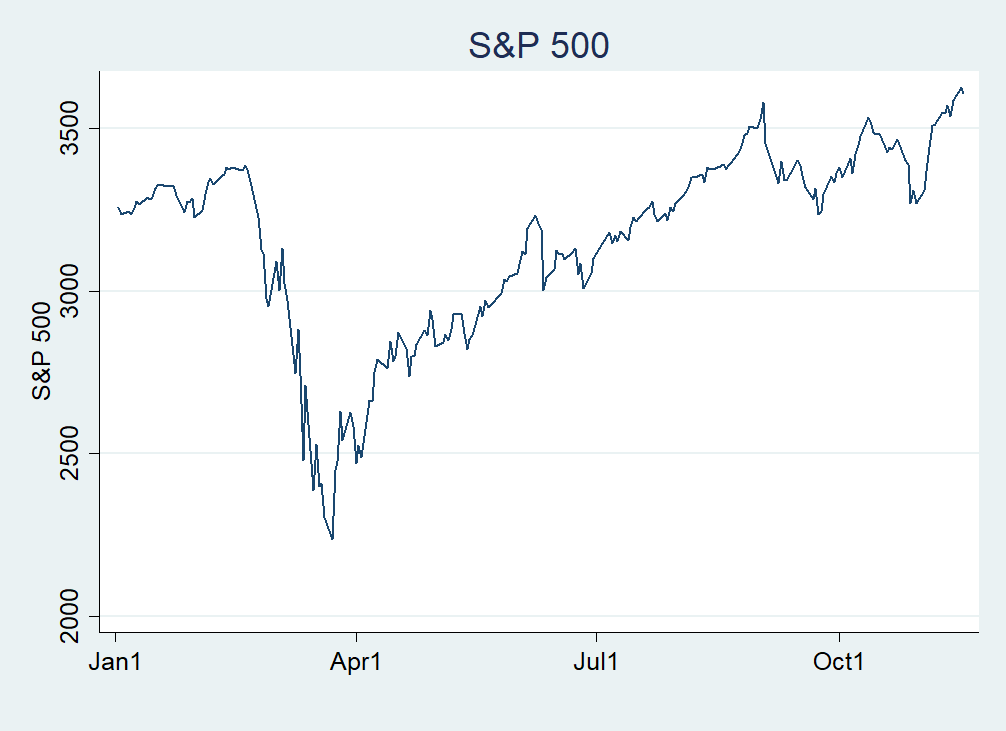
\includegraphics[height=6cm ]{\FigDir/sp500.png}
	\end{figure}
	%\begin{figure}[ht]
	\centering
	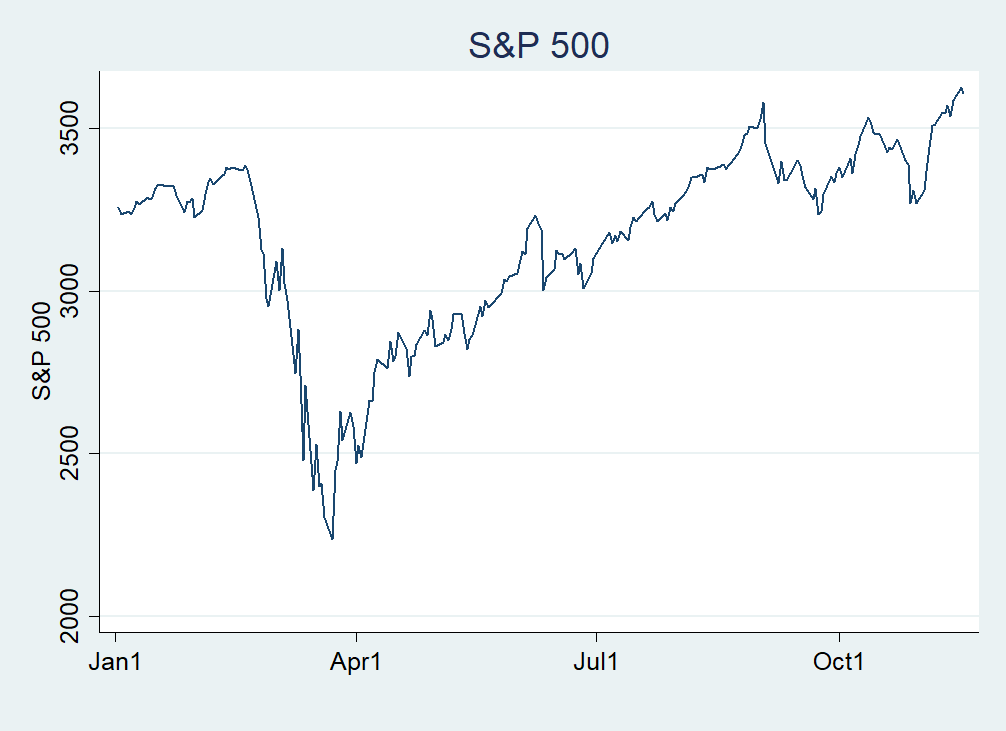
\includegraphics[height=6cm ]{\FigDir/sp500.png}
\end{figure}
	%\vspace{-1em}
	\hyperlink{motivation_2}{\beamerbutton{back}}
\end{frame}

\begin{frame}[label = eurostoxx50, noframenumbering]
	\frametitle{Motivation (2): Stock market turbulence due to Covid-19}
	\begin{figure}
		\centering
		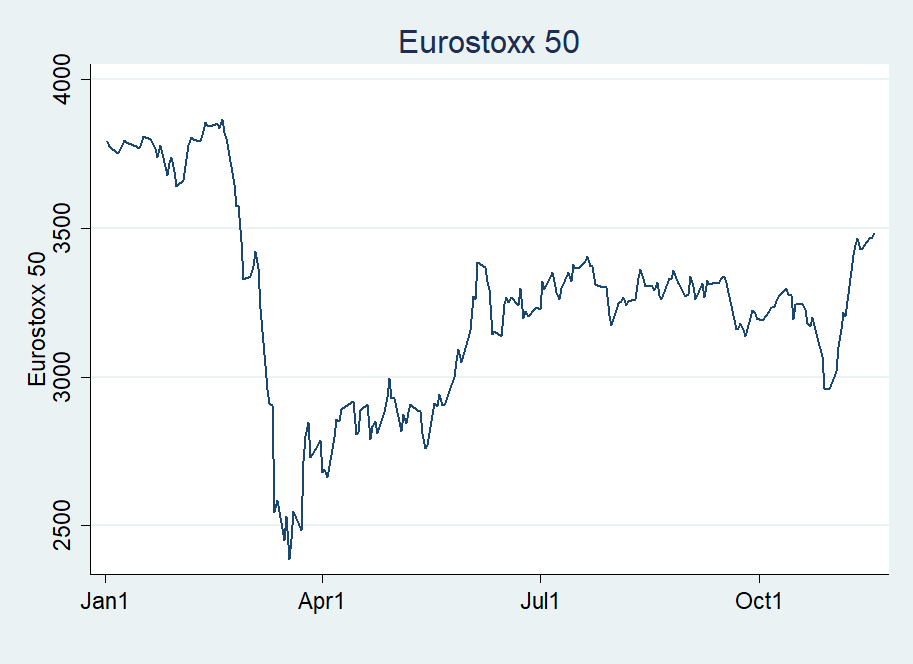
\includegraphics[height=6cm ]{\FigDir/eurostoxx50.png}
	\end{figure}
	%\begin{figure}
	\centering
	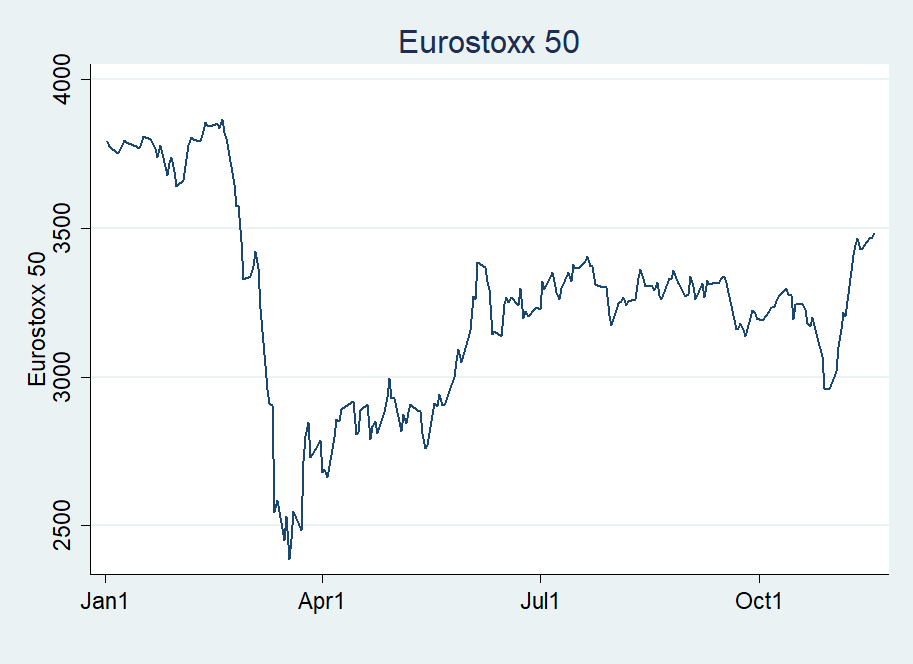
\includegraphics[height=6cm ]{\FigDir/eurostoxx50.png}
\end{figure}
	%\vspace{-1em}
	\hyperlink{motivation_2}{\beamerbutton{back}}
\end{frame}


\begin{frame}[label = BOP Q1, noframenumbering]
	\frametitle{BOP Questions (1)}
	\hyperlink{Timeline}{\beamerbutton{back}}
	\centering
	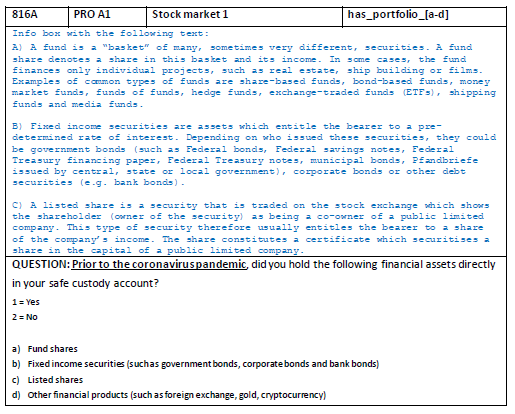
\includegraphics[height=7cm]{\FigDir/Q1_full.PNG}
\end{frame}

\begin{frame}[label = BOP Q2, noframenumbering]
	\frametitle{BOP Questions (2)}
	\hyperlink{Timeline}{\beamerbutton{back}}
	\centering
	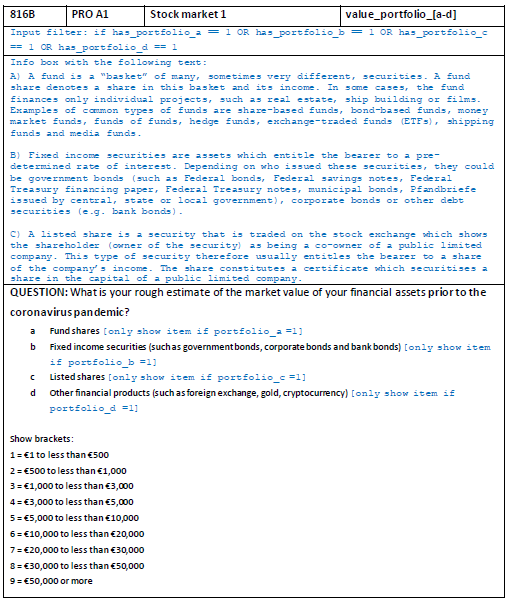
\includegraphics[height=7cm]{\FigDir/Q2_full.PNG}
\end{frame}

\begin{frame}[label = BOP Q3, noframenumbering]
	\frametitle{BOP Questions (3)}
	\hyperlink{Timeline}{\beamerbutton{back}}
	\centering
	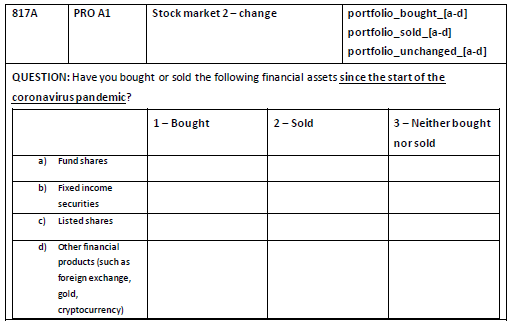
\includegraphics[height=7cm]{\FigDir/Q3_full.PNG}
\end{frame}

\begin{frame}[label = BOP Q4, noframenumbering]
	\frametitle{BOP Questions (4)}
	\hyperlink{Timeline}{\beamerbutton{back}}
	\centering
	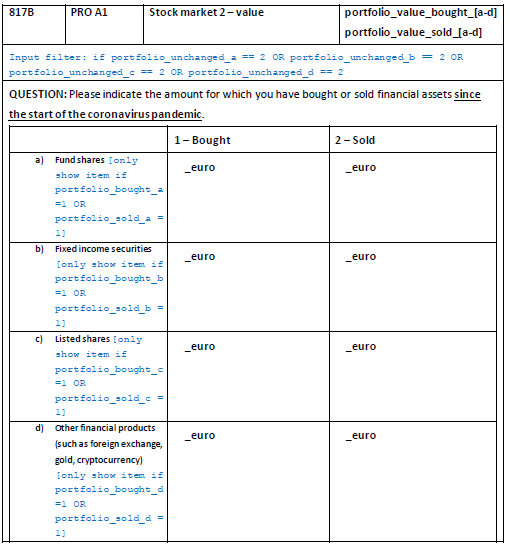
\includegraphics[height=7cm]{\FigDir/Q4_full.PNG}
\end{frame}

\begin{frame}[label = BOP Q5, noframenumbering]
	\frametitle{BOP Questions (5)}
	\hyperlink{Data}{\beamerbutton{back}}
	\centering
	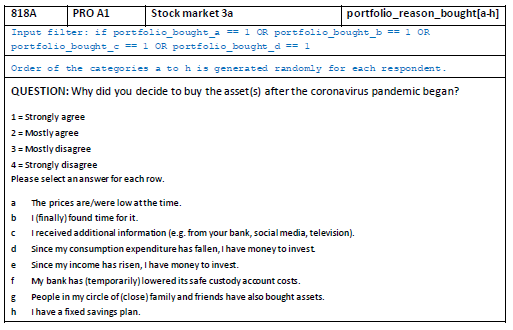
\includegraphics[height=7cm]{\FigDir/Q5_full.PNG}
\end{frame}

\begin{frame}[label = BOP Q6, noframenumbering]
	\frametitle{BOP Questions (6)}
	\hyperlink{Data}{\beamerbutton{back}}
	\centering
	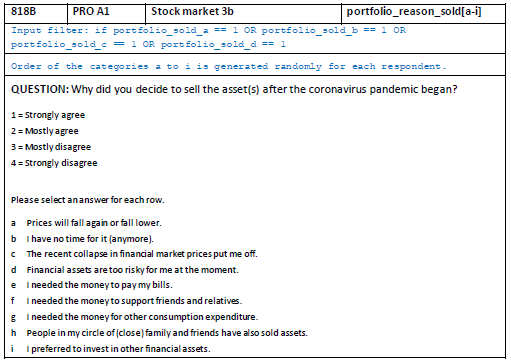
\includegraphics[height=7cm]{\FigDir/Q6_full.PNG}
\end{frame}

\begin{frame}[label = BOP Q7, noframenumbering]
	\frametitle{BOP Questions (7)}
	\hyperlink{Data}{\beamerbutton{back}}
	\centering
	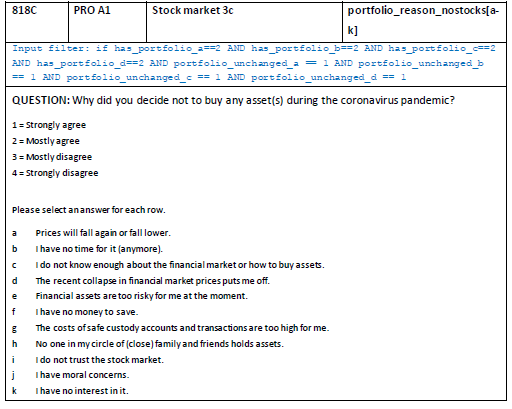
\includegraphics[height=7cm]{\FigDir/Q7_full.PNG}
\end{frame}

\begin{frame}[label = BOP Q8, noframenumbering]
	\frametitle{BOP Questions (8)}
	\hyperlink{Data}{\beamerbutton{back}}
	\centering
	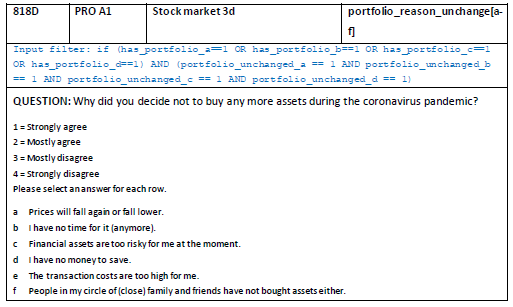
\includegraphics[height=7cm]{\FigDir/Q8_full.PNG}
\end{frame}


%%%%%%%%%%%%%%%%%%%%%%%%%%%%%%%%%%%%%%%%%%%%%%%%%%%%%%%%%%%%%%%%%%

\begin{frame}[plain, label = regression_nopart_dem, noframenumbering]
	\begin{table}[] \centering
		\resizebox{1.2\textheight}{!}{%
			\begin{threeparttable}
				\begin{tabular}{l*{11}{c}}
					\hline\hline
					                    &\multicolumn{1}{c}{(1)}&\multicolumn{1}{c}{(2)}&\multicolumn{1}{c}{(3)}&\multicolumn{1}{c}{(4)}&\multicolumn{1}{c}{(5)}&\multicolumn{1}{c}{(6)}&\multicolumn{1}{c}{(7)}&\multicolumn{1}{c}{(8)}&\multicolumn{1}{c}{(9)}&\multicolumn{1}{c}{(10)}&\multicolumn{1}{c}{(11)}\\
                    &\multicolumn{1}{c}{\shortstack{no information}}&\multicolumn{1}{c}{\shortstack{no interest}}&\multicolumn{1}{c}{\shortstack{distrust}}&\multicolumn{1}{c}{\shortstack{too risky}}&\multicolumn{1}{c}{\shortstack{no time}}&\multicolumn{1}{c}{\shortstack{peer-effect}}&\multicolumn{1}{c}{\shortstack{no savings}}&\multicolumn{1}{c}{\shortstack{prices fall}}&\multicolumn{1}{c}{\shortstack{shock}}&\multicolumn{1}{c}{\shortstack{cost}}&\multicolumn{1}{c}{\shortstack{moral}}\\
\hline
college             &       0.021         &       0.163         &      -0.051         &       0.032         &       0.163\sym{*}  &      -0.113         &      -0.107         &      -0.076         &      -0.074         &      -0.012         &       0.061         \\
                    &     (0.082)         &     (0.100)         &     (0.078)         &     (0.081)         &     (0.096)         &     (0.110)         &     (0.133)         &     (0.085)         &     (0.093)         &     (0.098)         &     (0.099)         \\
[1em]
full-time           &       0.119         &       0.044         &      -0.013         &       0.077         &       0.294\sym{**} &       0.228         &      -0.260         &      -0.045         &      -0.079         &       0.030         &      -0.373\sym{**} \\
                    &     (0.117)         &     (0.159)         &     (0.121)         &     (0.129)         &     (0.131)         &     (0.164)         &     (0.193)         &     (0.134)         &     (0.136)         &     (0.125)         &     (0.154)         \\
[1em]
part-time           &       0.095         &       0.244         &      -0.036         &       0.038         &       0.092         &       0.137         &      -0.329         &      -0.083         &      -0.115         &       0.051         &      -0.058         \\
                    &     (0.134)         &     (0.162)         &     (0.136)         &     (0.131)         &     (0.179)         &     (0.186)         &     (0.224)         &     (0.146)         &     (0.144)         &     (0.139)         &     (0.168)         \\
[1em]
retired             &       0.072         &       0.222         &      -0.100         &      -0.078         &       0.029         &       0.136         &      -0.126         &       0.248         &      -0.085         &       0.122         &      -0.385\sym{**} \\
                    &     (0.179)         &     (0.198)         &     (0.142)         &     (0.184)         &     (0.179)         &     (0.208)         &     (0.229)         &     (0.156)         &     (0.177)         &     (0.177)         &     (0.191)         \\
[1em]
self-employed       &      -0.300         &       0.001         &      -0.248         &       0.005         &       0.391\sym{**} &       0.079         &      -0.300         &       0.488\sym{**} &       0.116         &       0.102         &      -0.301         \\
                    &     (0.229)         &     (0.281)         &     (0.171)         &     (0.180)         &     (0.196)         &     (0.211)         &     (0.432)         &     (0.229)         &     (0.215)         &     (0.239)         &     (0.239)         \\
[1em]
female              &       0.071         &       0.161\sym{*}  &      -0.015         &      -0.078         &       0.139\sym{*}  &      -0.135         &      -0.006         &      -0.047         &       0.018         &      -0.029         &      -0.108         \\
                    &     (0.079)         &     (0.088)         &     (0.078)         &     (0.078)         &     (0.081)         &     (0.101)         &     (0.118)         &     (0.082)         &     (0.084)         &     (0.082)         &     (0.093)         \\
[1em]
short-time work     &       0.241\sym{*}  &       0.249         &       0.092         &      -0.143         &      -0.226         &      -0.129         &      -0.392         &       0.152         &       0.298         &      -0.284         &       0.183         \\
                    &     (0.137)         &     (0.197)         &     (0.149)         &     (0.165)         &     (0.177)         &     (0.167)         &     (0.291)         &     (0.133)         &     (0.217)         &     (0.188)         &     (0.217)         \\
[1em]
children            &      -0.119         &       0.092         &       0.124         &      -0.167\sym{*}  &       0.157         &       0.001         &       0.242\sym{*}  &      -0.139         &      -0.067         &      -0.155         &      -0.024         \\
                    &     (0.087)         &     (0.111)         &     (0.092)         &     (0.098)         &     (0.107)         &     (0.123)         &     (0.139)         &     (0.103)         &     (0.098)         &     (0.102)         &     (0.115)         \\
[1em]
1500-3000           &      -0.079         &       0.226\sym{*}  &      -0.067         &       0.207\sym{*}  &       0.060         &       0.026         &      -0.199         &       0.129         &      -0.030         &      -0.050         &      -0.202         \\
                    &     (0.118)         &     (0.133)         &     (0.115)         &     (0.117)         &     (0.129)         &     (0.148)         &     (0.186)         &     (0.111)         &     (0.124)         &     (0.124)         &     (0.156)         \\
[1em]
3000-5000           &      -0.047         &       0.246         &      -0.019         &       0.269\sym{**} &       0.050         &       0.049         &      -0.589\sym{***}&       0.138         &      -0.028         &      -0.000         &      -0.045         \\
                    &     (0.126)         &     (0.149)         &     (0.127)         &     (0.118)         &     (0.140)         &     (0.149)         &     (0.221)         &     (0.118)         &     (0.117)         &     (0.135)         &     (0.177)         \\
[1em]
5000-8000           &       0.069         &       0.427\sym{**} &      -0.009         &       0.092         &       0.082         &      -0.170         &      -0.695\sym{***}&       0.269         &       0.108         &       0.028         &      -0.161         \\
                    &     (0.153)         &     (0.187)         &     (0.150)         &     (0.138)         &     (0.177)         &     (0.193)         &     (0.255)         &     (0.168)         &     (0.137)         &     (0.150)         &     (0.179)         \\
[1em]
8000+               &      -0.278         &       0.522\sym{**} &       0.151         &       0.452\sym{***}&      -0.032         &      -0.410         &      -0.458         &       0.077         &       0.139         &       0.204         &      -0.413\sym{*}  \\
                    &     (0.177)         &     (0.204)         &     (0.171)         &     (0.151)         &     (0.279)         &     (0.326)         &     (0.278)         &     (0.186)         &     (0.209)         &     (0.218)         &     (0.211)         \\
[1em]
owner               &      -0.038         &       0.035         &      -0.003         &       0.028         &       0.010         &      -0.009         &      -0.065         &       0.089         &       0.051         &      -0.074         &      -0.035         \\
                    &     (0.075)         &     (0.094)         &     (0.075)         &     (0.082)         &     (0.089)         &     (0.099)         &     (0.125)         &     (0.085)         &     (0.082)         &     (0.085)         &     (0.105)         \\
[1em]
age                 &      -0.014\sym{***}&      -0.001         &       0.010\sym{***}&       0.009\sym{**} &      -0.014\sym{***}&       0.003         &      -0.005         &      -0.003         &       0.010\sym{**} &       0.003         &       0.001         \\
                    &     (0.003)         &     (0.004)         &     (0.003)         &     (0.004)         &     (0.004)         &     (0.004)         &     (0.005)         &     (0.004)         &     (0.004)         &     (0.003)         &     (0.004)         \\
[1em]
fin illiterate      &       0.261\sym{**} &       0.035         &      -0.133         &      -0.067         &       0.005         &      -0.052         &      -0.292\sym{**} &      -0.041         &       0.129         &       0.029         &       0.121         \\
                    &     (0.103)         &     (0.119)         &     (0.112)         &     (0.127)         &     (0.129)         &     (0.172)         &     (0.129)         &     (0.119)         &     (0.155)         &     (0.144)         &     (0.139)         \\
\hline
Observations        &         838         &         837         &         833         &         824         &         829         &         831         &         837         &         817         &         819         &         812         &         829         \\
Adjusted \(R^{2}\)  &       0.087         &       0.031         &       0.022         &       0.049         &       0.109         &       0.015         &       0.054         &       0.031         &       0.031         &       0.012         &       0.023         \\

					\hline\hline
				\end{tabular}
			\end{threeparttable}
		}
	\end{table}
	\hyperlink{results_nopart}{\beamerbutton{back}}
\end{frame}

\begin{frame}[plain,label = regression_pca_noadjust_dem_control, noframenumbering]
	\begin{table}[] \centering
		\resizebox{0.6\textheight}{!}{%
			\begin{threeparttable}
				\begin{tabular}{l*{6}c}
					\hline\hline
					                    &            &\multicolumn{1}{c}{(1)}&            &\multicolumn{1}{c}{(2)}&            &\multicolumn{1}{c}{(3)}\\
                    &            &\multicolumn{1}{c}{\shortstack{Risk \\ Aversion}}&            &\multicolumn{1}{c}{\shortstack{Lack of \\ Resources}}&            &\multicolumn{1}{c}{\shortstack{Lack of\\ Savings}}\\
\hline
college             &            &      -0.034         &            &       0.060         &            &      -0.053         \\
                    &            &     (0.049)         &            &     (0.048)         &            &     (0.070)         \\
[1em]
female              &            &      -0.034         &            &       0.089\sym{*}  &            &      -0.049         \\
                    &            &     (0.044)         &            &     (0.046)         &            &     (0.063)         \\
[1em]
children            &            &      -0.046         &            &       0.086         &            &       0.090         \\
                    &            &     (0.058)         &            &     (0.056)         &            &     (0.078)         \\
[1em]
owner               &            &       0.057         &            &      -0.033         &            &      -0.103         \\
                    &            &     (0.046)         &            &     (0.047)         &            &     (0.063)         \\
[1em]
fin illiterate      &            &      -0.025         &            &       0.007         &            &      -0.080         \\
                    &            &     (0.078)         &            &     (0.060)         &            &     (0.088)         \\
[1em]
part-time           &            &      -0.052         &            &       0.034         &            &      -0.201         \\
                    &            &     (0.078)         &            &     (0.086)         &            &     (0.126)         \\
[1em]
retired             &            &      -0.025         &            &       0.071         &            &      -0.223         \\
                    &            &     (0.092)         &            &     (0.104)         &            &     (0.138)         \\
[1em]
self-employed       &            &       0.076         &            &      -0.052         &            &      -0.296         \\
                    &            &     (0.110)         &            &     (0.138)         &            &     (0.201)         \\
[1em]
kurzarbeit          &            &       0.081         &            &      -0.021         &            &      -0.049         \\
                    &            &     (0.109)         &            &     (0.110)         &            &     (0.154)         \\
[1em]
age                 &            &       0.006\sym{***}&            &      -0.009\sym{***}&            &      -0.002         \\
                    &            &     (0.002)         &            &     (0.002)         &            &     (0.003)         \\
[1em]
$<1500$             &            &      -0.073         &            &       0.029         &            &       0.261\sym{***}\\
                    &            &     (0.058)         &            &     (0.064)         &            &     (0.096)         \\
\hline
Observations        &            &         811         &            &         823         &            &         827         \\
Adjusted \(R^{2}\)  &            &       0.073         &            &       0.103         &            &       0.059         \\

					\hline\hline
				\end{tabular}
			\end{threeparttable}
		}
	\end{table}
	\hyperlink{regression_pca_noadjust_dem}{\beamerbutton{back}}
\end{frame}

%%%%%%%%%%%%%%%%%%%%%%%%%%%%%%%%%%%%%%%%%%%%%%%%%%%%%%%%%%%%%%%%%%
\begin{frame}[plain, label = regression_noadjust_dem, noframenumbering]
	\begin{table}[] \centering
		\resizebox{0.8\textheight}{!}{%
			\begin{threeparttable}
				\begin{tabular}{l*{14}{c}}
					\hline\hline
					                    &            &\multicolumn{1}{c}{(1)}&            &\multicolumn{1}{c}{(2)}&            &\multicolumn{1}{c}{(3)}&            &\multicolumn{1}{c}{(4)}&            &\multicolumn{1}{c}{(5)}&            &\multicolumn{1}{c}{(6)}\\
                    &            &\multicolumn{1}{c}{\shortstack{too risky}}&            &\multicolumn{1}{c}{\shortstack{no time}}&            &\multicolumn{1}{c}{\shortstack{prices fall}}&            &\multicolumn{1}{c}{\shortstack{no savings}}&            &\multicolumn{1}{c}{\shortstack{peer effect}}&            &\multicolumn{1}{c}{\shortstack{costs}}\\
\hline
college             &            &      -0.061         &            &       0.334\sym{**} &            &      -0.151         &            &       0.037         &            &      -0.182         &            &       0.025         \\
                    &            &     (0.116)         &            &     (0.148)         &            &     (0.114)         &            &     (0.149)         &            &     (0.123)         &            &     (0.101)         \\
[1em]
full-time           &            &       0.235         &            &       0.277         &            &      -0.242         &            &      -0.322         &            &      -0.007         &            &       0.039         \\
                    &            &     (0.185)         &            &     (0.237)         &            &     (0.174)         &            &     (0.291)         &            &     (0.252)         &            &     (0.144)         \\
[1em]
part-time           &            &       0.128         &            &       0.033         &            &      -0.535\sym{*}  &            &       0.194         &            &       0.123         &            &       0.040         \\
                    &            &     (0.222)         &            &     (0.257)         &            &     (0.273)         &            &     (0.389)         &            &     (0.281)         &            &     (0.181)         \\
[1em]
retired             &            &       0.107         &            &      -0.142         &            &      -0.415\sym{*}  &            &      -0.365         &            &       0.673\sym{**} &            &       0.125         \\
                    &            &     (0.240)         &            &     (0.274)         &            &     (0.217)         &            &     (0.322)         &            &     (0.264)         &            &     (0.184)         \\
[1em]
self-employed       &            &      -0.242         &            &       0.076         &            &      -0.652\sym{***}&            &       0.438         &            &       0.139         &            &       0.230         \\
                    &            &     (0.250)         &            &     (0.338)         &            &     (0.226)         &            &     (0.344)         &            &     (0.266)         &            &     (0.349)         \\
[1em]
female              &            &      -0.001         &            &       0.084         &            &      -0.116         &            &      -0.148         &            &       0.038         &            &       0.142         \\
                    &            &     (0.104)         &            &     (0.138)         &            &     (0.137)         &            &     (0.145)         &            &     (0.139)         &            &     (0.097)         \\
[1em]
short-time work     &            &      -0.106         &            &      -0.148         &            &      -0.542\sym{***}&            &       0.051         &            &       0.468         &            &       0.262         \\
                    &            &     (0.255)         &            &     (0.265)         &            &     (0.165)         &            &     (0.242)         &            &     (0.323)         &            &     (0.334)         \\
[1em]
children            &            &       0.119         &            &       0.179         &            &      -0.244\sym{*}  &            &       0.196         &            &      -0.175         &            &      -0.073         \\
                    &            &     (0.150)         &            &     (0.184)         &            &     (0.129)         &            &     (0.206)         &            &     (0.173)         &            &     (0.129)         \\
[1em]
1500-3000           &            &      -0.240         &            &       0.161         &            &       0.259         &            &      -0.714\sym{***}&            &       0.175         &            &       0.379\sym{*}  \\
                    &            &     (0.189)         &            &     (0.274)         &            &     (0.202)         &            &     (0.270)         &            &     (0.245)         &            &     (0.199)         \\
[1em]
3000-5000           &            &       0.026         &            &       0.021         &            &       0.183         &            &      -0.862\sym{***}&            &       0.353         &            &       0.304         \\
                    &            &     (0.186)         &            &     (0.272)         &            &     (0.237)         &            &     (0.285)         &            &     (0.244)         &            &     (0.198)         \\
[1em]
5000-8000           &            &      -0.355         &            &       0.220         &            &       0.274         &            &      -0.728\sym{**} &            &       0.508\sym{*}  &            &       0.098         \\
                    &            &     (0.225)         &            &     (0.318)         &            &     (0.261)         &            &     (0.319)         &            &     (0.260)         &            &     (0.207)         \\
[1em]
8000+               &            &       0.358         &            &       0.598\sym{*}  &            &       0.031         &            &      -1.364\sym{***}&            &       0.169         &            &       0.213         \\
                    &            &     (0.264)         &            &     (0.323)         &            &     (0.269)         &            &     (0.385)         &            &     (0.319)         &            &     (0.285)         \\
[1em]
owner               &            &      -0.029         &            &      -0.088         &            &       0.324\sym{*}  &            &      -0.211         &            &      -0.166         &            &       0.167\sym{*}  \\
                    &            &     (0.117)         &            &     (0.136)         &            &     (0.170)         &            &     (0.158)         &            &     (0.136)         &            &     (0.100)         \\
[1em]
age                 &            &       0.006         &            &      -0.009\sym{*}  &            &       0.004         &            &       0.015\sym{**} &            &      -0.019\sym{***}&            &       0.004         \\
                    &            &     (0.005)         &            &     (0.006)         &            &     (0.005)         &            &     (0.007)         &            &     (0.007)         &            &     (0.004)         \\
[1em]
fin illiterate      &            &       0.292\sym{*}  &            &       0.303\sym{*}  &            &       0.209         &            &      -0.944\sym{***}&            &       0.406\sym{*}  &            &      -0.255\sym{**} \\
                    &            &     (0.164)         &            &     (0.167)         &            &     (0.205)         &            &     (0.324)         &            &     (0.241)         &            &     (0.117)         \\
\hline
Observations        &            &         440         &            &         441         &            &         436         &            &         439         &            &         432         &            &         437         \\
Adjusted \(R^{2}\)  &            &       0.038         &            &       0.124         &            &       0.097         &            &       0.112         &            &       0.073         &            &       0.046         \\

					\hline\hline
				\end{tabular}
			\end{threeparttable}
		}
	\end{table}
	\hyperlink{results_noadjust}{\beamerbutton{back}}
\end{frame}

%%%%%%%%%%%%%%%%%%%%%%%%%%%%%%%%%%%%%%%%%%%%%%%%%%%%%%%%%%%%%%%%%%
\begin{frame}[plain, label = regression_bought_dem, noframenumbering]
	\begin{table}[] \centering
		\resizebox{\textheight}{!}{%
			\begin{threeparttable}
				\begin{tabular}{l*{16}{c}}
					\hline\hline
					                    &\multicolumn{1}{c}{(1)}&\multicolumn{1}{c}{(2)}&\multicolumn{1}{c}{(3)}&\multicolumn{1}{c}{(4)}&\multicolumn{1}{c}{(5)}&\multicolumn{1}{c}{(6)}&\multicolumn{1}{c}{(7)}\\
                    &\multicolumn{1}{c}{\shortstack{low valuation}}&\multicolumn{1}{c}{\shortstack{plan}}&\multicolumn{1}{c}{\shortstack{time}}&\multicolumn{1}{c}{\shortstack{information}}&\multicolumn{1}{c}{\shortstack{less consumption}}&\multicolumn{1}{c}{\shortstack{more income}}&\multicolumn{1}{c}{\shortstack{peer effect}}\\
\hline
college             &      -0.067         &       0.100         &      -0.164         &      -0.060         &       0.042         &      -0.052         &       0.196\sym{**} \\
                    &     (0.121)         &     (0.150)         &     (0.102)         &     (0.110)         &     (0.084)         &     (0.086)         &     (0.089)         \\
[1em]
1500-3000           &      -0.801\sym{**} &       0.695\sym{*}  &       0.092         &      -0.073         &       0.503\sym{***}&       0.174         &      -0.590\sym{*}  \\
                    &     (0.316)         &     (0.376)         &     (0.267)         &     (0.377)         &     (0.161)         &     (0.283)         &     (0.346)         \\
[1em]
3000-5000           &      -0.594\sym{*}  &       0.903\sym{**} &       0.142         &      -0.126         &       0.357\sym{**} &      -0.094         &      -0.534         \\
                    &     (0.329)         &     (0.403)         &     (0.272)         &     (0.376)         &     (0.149)         &     (0.270)         &     (0.345)         \\
[1em]
5000-8000           &      -0.264         &       0.531         &       0.127         &      -0.245         &       0.335\sym{*}  &       0.093         &      -0.480         \\
                    &     (0.327)         &     (0.402)         &     (0.286)         &     (0.374)         &     (0.171)         &     (0.276)         &     (0.347)         \\
[1em]
8000+               &      -0.214         &       0.276         &      -0.139         &      -0.323         &       0.392\sym{*}  &       0.110         &       0.093         \\
                    &     (0.359)         &     (0.431)         &     (0.286)         &     (0.419)         &     (0.208)         &     (0.305)         &     (0.374)         \\
[1em]
$<30$               &       0.000         &       0.000         &       0.000         &       0.000         &       0.000         &       0.000         &       0.000         \\
                    &         (.)         &         (.)         &         (.)         &         (.)         &         (.)         &         (.)         &         (.)         \\
[1em]
31-40               &      -0.191         &       0.323         &      -0.493\sym{***}&       0.146         &       0.028         &       0.258         &      -0.340\sym{**} \\
                    &     (0.213)         &     (0.249)         &     (0.168)         &     (0.231)         &     (0.162)         &     (0.171)         &     (0.145)         \\
[1em]
41-50               &      -0.236         &       0.650\sym{***}&      -0.355\sym{*}  &      -0.135         &       0.021         &       0.111         &      -0.475\sym{***}\\
                    &     (0.164)         &     (0.244)         &     (0.190)         &     (0.175)         &     (0.134)         &     (0.142)         &     (0.138)         \\
[1em]
51-60               &      -0.523\sym{***}&       0.463\sym{*}  &      -0.282         &       0.140         &      -0.035         &       0.161         &      -0.379\sym{***}\\
                    &     (0.194)         &     (0.275)         &     (0.206)         &     (0.207)         &     (0.138)         &     (0.156)         &     (0.140)         \\
[1em]
60+                 &      -0.499\sym{*}  &       0.544\sym{*}  &      -0.264         &       0.440\sym{*}  &      -0.223         &      -0.039         &      -0.434\sym{**} \\
                    &     (0.270)         &     (0.288)         &     (0.243)         &     (0.230)         &     (0.186)         &     (0.152)         &     (0.175)         \\
[1em]
first time          &       0.195         &      -0.868\sym{***}&       0.688\sym{***}&       0.045         &      -0.266\sym{***}&       0.382\sym{*}  &      -0.070         \\
                    &     (0.202)         &     (0.271)         &     (0.185)         &     (0.236)         &     (0.102)         &     (0.223)         &     (0.251)         \\
[1em]
bought \& sold      &       0.518\sym{***}&      -0.957\sym{***}&       0.217         &       0.461\sym{***}&      -0.165\sym{*}  &      -0.017         &       0.013         \\
                    &     (0.131)         &     (0.175)         &     (0.132)         &     (0.172)         &     (0.092)         &     (0.094)         &     (0.100)         \\
\hline
Observations        &         435         &         438         &         438         &         437         &         438         &         438         &         434         \\
Controls            &         Yes         &         Yes         &         Yes         &         Yes         &         Yes         &         Yes         &         Yes         \\

					\hline\hline
				\end{tabular}
			\end{threeparttable}
		}
	\end{table}
	\hyperlink{results_bought}{\beamerbutton{back}}
\end{frame}

%%%%%%%%%%%%%%%%%%%%%%%%%%%%%%%%%%%%%%%%%%%%%%%%%%%%%%%%%%%%%%%%%%
\begin{frame}[plain, label = regression_sold_dem, noframenumbering]
	\begin{table}[] \centering
		\resizebox{\textheight}{!}{%
			\begin{threeparttable}
				\begin{tabular}{l*{18}{c}}
					\hline\hline
					                    &            &\multicolumn{1}{c}{(1)}&            &\multicolumn{1}{c}{(2)}&            &\multicolumn{1}{c}{(3)}&            &\multicolumn{1}{c}{(4)}&            &\multicolumn{1}{c}{(5)}&            &\multicolumn{1}{c}{(6)}&            &\multicolumn{1}{c}{(7)}&            &\multicolumn{1}{c}{(8)}&            &\multicolumn{1}{c}{(9)}\\
                    &            &\multicolumn{1}{c}{\shortstack{prices fall}}&            &\multicolumn{1}{c}{\shortstack{no time}}&            &\multicolumn{1}{c}{\shortstack{shock}}&            &\multicolumn{1}{c}{\shortstack{too risky}}&            &\multicolumn{1}{c}{\shortstack{need consumption}}&            &\multicolumn{1}{c}{\shortstack{need debt obligation}}&            &\multicolumn{1}{c}{\shortstack{no time}}&            &\multicolumn{1}{c}{\shortstack{peer-effect}}&            &\multicolumn{1}{c}{\shortstack{need support \\ friends and family}}\\
\hline
college             &            &       0.295         &            &       0.122         &            &      -0.250         &            &       0.279\sym{*}  &            &      -0.539\sym{**} &            &      -0.347\sym{*}  &            &       0.070         &            &       0.525\sym{***}&            &      -0.156\sym{*}  \\
                    &            &     (0.270)         &            &     (0.282)         &            &     (0.183)         &            &     (0.167)         &            &     (0.228)         &            &     (0.177)         &            &     (0.156)         &            &     (0.162)         &            &     (0.092)         \\
[1em]
part-time           &            &       0.513         &            &      -0.217         &            &       0.239         &            &       0.001         &            &      -0.278         &            &       0.325         &            &      -0.103         &            &      -0.426         &            &      -0.054         \\
                    &            &     (0.707)         &            &     (0.821)         &            &     (0.440)         &            &     (0.535)         &            &     (0.641)         &            &     (0.659)         &            &     (0.458)         &            &     (0.338)         &            &     (0.284)         \\
[1em]
retired             &            &       0.647         &            &      -0.663         &            &       0.137         &            &      -0.338         &            &       0.337         &            &       0.106         &            &      -0.443         &            &       0.032         &            &       0.186         \\
                    &            &     (0.596)         &            &     (0.701)         &            &     (0.480)         &            &     (0.455)         &            &     (0.545)         &            &     (0.572)         &            &     (0.485)         &            &     (0.377)         &            &     (0.316)         \\
[1em]
self-employed       &            &      -0.036         &            &       0.010         &            &       0.332         &            &      -0.269         &            &       0.661         &            &       0.065         &            &      -0.797\sym{*}  &            &      -0.196         &            &       0.230         \\
                    &            &     (0.546)         &            &     (0.740)         &            &     (0.441)         &            &     (0.473)         &            &     (0.719)         &            &     (0.544)         &            &     (0.437)         &            &     (0.332)         &            &     (0.277)         \\
[1em]
female              &            &       0.331         &            &       0.521         &            &      -0.306         &            &      -0.336\sym{*}  &            &       0.050         &            &      -0.178         &            &      -0.223         &            &       0.085         &            &       0.056         \\
                    &            &     (0.329)         &            &     (0.323)         &            &     (0.252)         &            &     (0.186)         &            &     (0.243)         &            &     (0.193)         &            &     (0.136)         &            &     (0.102)         &            &     (0.090)         \\
[1em]
kurzarbeit          &            &       0.038         &            &      -0.317         &            &      -0.635         &            &       0.021         &            &       0.223         &            &      -0.090         &            &      -0.430         &            &       0.933\sym{**} &            &       0.256         \\
                    &            &     (0.397)         &            &     (0.934)         &            &     (0.483)         &            &     (0.348)         &            &     (0.813)         &            &     (0.696)         &            &     (0.308)         &            &     (0.432)         &            &     (0.505)         \\
[1em]
children            &            &       0.159         &            &      -0.480         &            &      -0.200         &            &      -0.010         &            &       0.276         &            &       0.070         &            &      -0.011         &            &      -0.024         &            &       0.220\sym{**} \\
                    &            &     (0.297)         &            &     (0.343)         &            &     (0.224)         &            &     (0.211)         &            &     (0.258)         &            &     (0.256)         &            &     (0.162)         &            &     (0.140)         &            &     (0.105)         \\
[1em]
1500-3000           &            &       0.136         &            &       0.487         &            &      -0.200         &            &       0.105         &            &       0.529         &            &       0.366         &            &      -0.609         &            &      -0.666\sym{*}  &            &      -0.147         \\
                    &            &     (0.467)         &            &     (0.495)         &            &     (0.489)         &            &     (0.431)         &            &     (0.498)         &            &     (0.365)         &            &     (0.406)         &            &     (0.366)         &            &     (0.267)         \\
[1em]
3000-5000           &            &      -0.095         &            &       0.531         &            &      -0.178         &            &       0.117         &            &       0.614         &            &       0.544         &            &      -0.776\sym{*}  &            &      -0.554         &            &      -0.203         \\
                    &            &     (0.422)         &            &     (0.530)         &            &     (0.473)         &            &     (0.422)         &            &     (0.506)         &            &     (0.425)         &            &     (0.400)         &            &     (0.338)         &            &     (0.269)         \\
[1em]
5000-8000           &            &       0.508         &            &       0.346         &            &      -0.401         &            &       0.090         &            &       0.319         &            &       0.154         &            &      -0.278         &            &      -0.606\sym{*}  &            &      -0.131         \\
                    &            &     (0.480)         &            &     (0.542)         &            &     (0.490)         &            &     (0.448)         &            &     (0.523)         &            &     (0.404)         &            &     (0.425)         &            &     (0.362)         &            &     (0.285)         \\
[1em]
8000+               &            &       0.096         &            &      -0.063         &            &      -0.162         &            &       0.348         &            &       0.574         &            &       0.483         &            &      -0.682         &            &      -0.597         &            &       0.003         \\
                    &            &     (0.552)         &            &     (0.634)         &            &     (0.550)         &            &     (0.504)         &            &     (0.519)         &            &     (0.403)         &            &     (0.439)         &            &     (0.376)         &            &     (0.273)         \\
[1em]
owner               &            &       0.211         &            &      -0.109         &            &       0.197         &            &      -0.156         &            &      -0.095         &            &      -0.099         &            &       0.164         &            &      -0.015         &            &      -0.098         \\
                    &            &     (0.274)         &            &     (0.350)         &            &     (0.188)         &            &     (0.180)         &            &     (0.243)         &            &     (0.195)         &            &     (0.137)         &            &     (0.124)         &            &     (0.104)         \\
[1em]
age                 &            &       0.000         &            &      -0.004         &            &       0.015\sym{*}  &            &       0.020\sym{**} &            &      -0.014         &            &      -0.009         &            &      -0.001         &            &      -0.006         &            &      -0.000         \\
                    &            &     (0.013)         &            &     (0.018)         &            &     (0.008)         &            &     (0.009)         &            &     (0.012)         &            &     (0.009)         &            &     (0.006)         &            &     (0.006)         &            &     (0.005)         \\
[1em]
fin illiterate      &            &      -0.353         &            &       0.717         &            &       0.408         &            &      -0.100         &            &      -0.422         &            &       0.166         &            &       0.306         &            &      -1.172\sym{***}&            &       0.451         \\
                    &            &     (0.380)         &            &     (0.692)         &            &     (0.469)         &            &     (0.306)         &            &     (0.643)         &            &     (0.561)         &            &     (0.365)         &            &     (0.361)         &            &     (0.381)         \\
[1em]
bought \& sold      &            &       0.215         &            &       1.361\sym{***}&            &      -0.355         &            &      -0.570\sym{***}&            &      -0.226         &            &      -0.445\sym{**} &            &      -0.192         &            &       0.110         &            &       0.101         \\
                    &            &     (0.259)         &            &     (0.278)         &            &     (0.220)         &            &     (0.191)         &            &     (0.251)         &            &     (0.218)         &            &     (0.158)         &            &     (0.166)         &            &     (0.128)         \\
\hline
Observations        &            &         120         &            &         120         &            &         120         &            &         120         &            &         120         &            &         120         &            &         120         &            &         120         &            &         120         \\
Adjusted \(R^{2}\)  &            &       0.075         &            &       0.192         &            &       0.095         &            &       0.148         &            &       0.028         &            &       0.059         &            &       0.236         &            &       0.256         &            &       0.092         \\

					\hline\hline
				\end{tabular}
			\end{threeparttable}
		}
	\end{table}
	\hyperlink{results_sold}{\beamerbutton{back}}
\end{frame}
%%%%%%%%%%%%%%%%%%%%%%%%%%%%%%%%%%%%%%%%%%%%%%%%%%%%%%%%%%%%%%%%%%
\begin{frame}[label = regression_bought_expec_pp_cond, noframenumbering]
	\frametitle{House Price Expectations and Buyer}
	\vspace{-1em}
	\begin{table}[htbp]\centering
		\resizebox{\textwidth}{!}{%
			\begin{tabular}{l*{6}{c}}
				\hline\hline
				                    &\multicolumn{1}{c}{(1)}&\multicolumn{1}{c}{(2)}&\multicolumn{1}{c}{(3)}&\multicolumn{1}{c}{(4)}&\multicolumn{1}{c}{(5)}&\multicolumn{1}{c}{(6)}\\
                    &\multicolumn{1}{c}{\shortstack{All}}&\multicolumn{1}{c}{\shortstack{Owner}}&\multicolumn{1}{c}{\shortstack{Renter}}&\multicolumn{1}{c}{\shortstack{All}}&\multicolumn{1}{c}{\shortstack{Owner}}&\multicolumn{1}{c}{\shortstack{Renter}}\\
\hline
                    &                     &                     &                     &                     &                     &                     \\
housing quali       &      -0.130\sym{**} &                     &                     &                     &                     &                     \\
                    &     (0.059)         &                     &                     &                     &                     &                     \\
[1em]
prop quali          &                     &      -0.127\sym{*}  &                     &                     &                     &                     \\
                    &                     &     (0.068)         &                     &                     &                     &                     \\
[1em]
rent quali          &                     &                     &      -0.122         &                     &                     &                     \\
                    &                     &                     &     (0.113)         &                     &                     &                     \\
[1em]
house price wins    &                     &                     &                     &      -0.029\sym{**} &       0.001         &      -0.084\sym{***}\\
                    &                     &                     &                     &     (0.011)         &     (0.013)         &     (0.020)         \\
\hline
Observations        &        1006         &         714         &         292         &         948         &         675         &         273         \\
Controls            &         Yes         &         Yes         &         Yes         &         Yes         &         Yes         &         Yes         \\

				\hline\hline
			\end{tabular}
		}
	\end{table}
	\hyperlink{regression_bought_expec_pp}{\beamerbutton{back}}
\end{frame}

\begin{frame}[label = regression_bought_infl_cond, noframenumbering]
	\frametitle{Inflation Expectations and Buyer}
	\vspace{-1em}
	\begin{table}[htbp]\centering
		\resizebox{0.9\textwidth}{!}{%
			\begin{tabular}{l*{8}{c}}
				\hline\hline
				                    &\multicolumn{1}{c}{(1)}         &\multicolumn{1}{c}{(2)}         &\multicolumn{1}{c}{(3)}         &\multicolumn{1}{c}{(4)}         &\multicolumn{1}{c}{(5)}         &\multicolumn{1}{c}{(6)}         &\multicolumn{1}{c}{(7)}         &\multicolumn{1}{c}{(8)}         \\
\hline
                    &                     &                     &                     &                     &                     &                     &                     &                     \\
inflation quali     &      -0.262\sym{***}&                     &                     &                     &                     &                     &                     &                     \\
                    &     (0.101)         &                     &                     &                     &                     &                     &                     &                     \\
[1em]
inflation PE wins   &                     &      -0.045\sym{***}&      -0.056\sym{***}&      -0.038\sym{**} &                     &                     &                     &                     \\
                    &                     &     (0.012)         &     (0.013)         &     (0.018)         &                     &                     &                     &                     \\
[1em]
fin illiterate:     &                     &                     &       0.441         &                     &                     &                     &                     &                     \\
inflation $>|30|$   &                     &                     &     (0.308)         &                     &                     &                     &                     &                     \\
[1em]
fin illiterate:     &                     &                     &                     &      -0.203         &                     &                     &                     &                     \\
inflation $>|10|$   &                     &                     &                     &     (0.371)         &                     &                     &                     &                     \\
[1em]
$0<$ inflation $<10$&                     &                     &                     &                     &      -0.117\sym{***}&                     &                     &                     \\
                    &                     &                     &                     &                     &     (0.030)         &                     &                     &                     \\
[1em]
$0<$ inflation $<5$ &                     &                     &                     &                     &                     &      -0.144\sym{***}&                     &                     \\
                    &                     &                     &                     &                     &                     &     (0.047)         &                     &                     \\
[1em]
inflation prob exp  &                     &                     &                     &                     &                     &                     &      -0.077\sym{***}&      -0.099\sym{***}\\
                    &                     &                     &                     &                     &                     &                     &     (0.020)         &     (0.026)         \\
[1em]
inflation prob sd   &                     &                     &                     &                     &                     &                     &                     &      -0.354         \\
                    &                     &                     &                     &                     &                     &                     &                     &     (0.247)         \\
\hline
Observations        &        1004         &        1006         &        1006         &        1006         &         950         &         884         &         892         &         892         \\
Controls            &         Yes         &         Yes         &         Yes         &         Yes         &         Yes         &         Yes         &         Yes         &         Yes         \\

				\hline\hline
			\end{tabular}
		}
	\end{table}
	\hyperlink{regression_bought_expec_infl}{\beamerbutton{back}}
\end{frame}

\begin{frame}[label = regression_expec_infl, noframenumbering]
	\frametitle{Inflation Expectations and Buyer}
	\vspace{-1em}
	\begin{table}[htbp]\centering
		\resizebox{0.9\textwidth}{!}{%
			\begin{tabular}{l*{10}{c}}
				\hline\hline
				                    &            &\multicolumn{1}{c}{(1)}&            &\multicolumn{1}{c}{(2)}&            &\multicolumn{1}{c}{(3)}&            &\multicolumn{1}{c}{(4)}&            &\multicolumn{1}{c}{(5)}\\
                    &            &\multicolumn{1}{c}{\shortstack{inflation}}&            &\multicolumn{1}{c}{\shortstack{inflation}}&            &\multicolumn{1}{c}{\shortstack{inflation}}&            &\multicolumn{1}{c}{\shortstack{Bought}}&            &\multicolumn{1}{c}{\shortstack{Bought}}\\
\hline
                    &            &                     &            &                     &            &                     &            &                     &            &                     \\
pess economy        &            &       0.280\sym{***}&            &                     &            &       0.279\sym{***}&            &                     &            &      -0.003         \\
                    &            &     (0.070)         &            &                     &            &     (0.071)         &            &                     &            &     (0.022)         \\
[1em]
inc interest rates  &            &                     &            &       0.452\sym{**} &            &       0.451\sym{**} &            &                     &            &      -0.103\sym{*}  \\
                    &            &                     &            &     (0.221)         &            &     (0.216)         &            &                     &            &     (0.060)         \\
[1em]
inflation PE wins   &            &                     &            &                     &            &                     &            &      -0.097\sym{***}&            &      -0.098\sym{***}\\
                    &            &                     &            &                     &            &                     &            &     (0.018)         &            &     (0.019)         \\
\hline
Observations        &            &        1883         &            &        1881         &            &        1881         &            &        1883         &            &        1881         \\
Controls            &            &         Yes         &            &         Yes         &            &         Yes         &            &         Yes         &            &         Yes         \\

				\hline\hline
			\end{tabular}
		}
	\end{table}
	\hyperlink{regression_bought_expec_infl}{\beamerbutton{back}}
\end{frame}

\end{document}\endinput

% Local Variables:
% eval: (setq TeX-command-list  (remove '("Biber" "biber %s" TeX-run-Biber nil  (plain-tex-mode latex-mode doctex-mode ams-tex-mode texinfo-mode)  :help "Run Biber") TeX-command-list))
% eval: (setq TeX-command-list  (remove '("BibTeX" "%(bibtex) %s" TeX-run-BibTeX nil t                                                                              :help "Run BibTeX") TeX-command-list))
% eval: (setq TeX-command-list  (remove '("BibTeX" "%(bibtex) %s" TeX-run-BibTeX nil (plain-tex-mode latex-mode doctex-mode ams-tex-mode texinfo-mode context-mode) :help "Run BibTeX") TeX-command-list))
% eval: (setq TeX-command-list  (remove '("BibTeX" "%(bibtex) ../LaTeX/%s" TeX-run-BibTeX nil t :help "Run BibTeX")   TeX-command-list))
% eval: (add-to-list 'TeX-command-list	'("BibTeX" "%(bibtex) LaTeX/%s" TeX-run-BibTeX nil t :help "Run BibTeX") t)
% eval: (cond ((string-equal system-type "darwin") (progn (setq TeX-view-program-list '(("Skim" "/Applications/Skim.app/Contents/SharedSupport/displayline -b %n LaTeX/%o %b"))))))
% TeX-PDF-mode: t
% TeX-file-line-error: t
% TeX-debug-warnings: t
% LaTeX-command-style: (("" "%(PDF)%(latex) %(file-line-error) %(extraopts) -output-directory=LaTeX %S%(PDFout)"))
% TeX-source-correlate-mode: t
% TeX-source-correlate-start-server: 0
% TeX-parse-self: t
% End:
